\documentclass[USenglish,oneside,twocolumn]{article}
\usepackage{color}
\usepackage[hyphens]{url}
\usepackage{longtable}
\usepackage{graphicx}
\usepackage{enumitem}
\usepackage{pdfpages}
%\usepackage{hyperref}

\usepackage[utf8]{inputenc}%(only for the pdftex engine)
%\RequirePackage[no-math]{fontspec}%(only for the luatex or the xetex engine)
\usepackage[big]{dgruyter_NEW}
 
\DOI{foobar}

\cclogo{
\includegraphics{by-nc-nd.pdf}}

% Format a participant quotation.
\newcommand{\pquote}[2]{
\begin{quotation}
\noindent #1:~\textit{``#2''}
\end{quotation}
}
  
\begin{document}
 
  \author*[1]{Linda Lee}

  \author[2]{David Fifield}

  \author[3]{Nathan Malkin}

  \author[4]{Ganesh Iyer}

  \author[5]{Serge Egelman}
  
  \author[6]{David Wagner}

  \affil[1]{University of California Berkeley, E-mail: \mbox{lnl@cs.berkeley.edu}}

  \affil[2]{University of California Berkeley, E-mail: \mbox{fifield@cs.berkeley.edu}}

  \affil[3]{University of California Berkeley, E-mail: \mbox{nmalkin@cs.berkeley.edu}}

  \affil[4]{University of California Berkeley, E-mail: \mbox{ganesh.v@berkeley.edu}}
  
  \affil[5]{University of California Berkeley and International Computer Science Institute, E-mail: \mbox{egelman@cs.berkeley.edu}}
   
  \affil[6]{University of California Berkeley, E-mail: \mbox{daw@cs.berkeley.edu}}

  \title{\huge Tor's Usability for Censorship Circumvention}
  %Internet Freedom Made Easy: On Improving Tor’s Usability for Censorship Circumvention
  %Towards Usable Censorship Circumvention

  \runningtitle{Tor's Usability for Censorship Circumvention}

  %\subtitle{...}

  \begin{abstract}
{Tor has grown beyond its original purpose as an anonymity tool and has 
become a widely-used censorship circumvention tool.
This is the first study to examine Tor's usability as a censorship circumvention tool.
We evaluate, redesign, and test the Tor configuration interface by
placing users in simulated censorship environments, instruct them to use Tor
to circumvent censorship, and measuring their interactions with the interface.
A 16-participant qualitative user study identifies common user struggles while circumventing censorship.
We use the results as feedback to redesign the configuration interface.
A 124-participant quantitative user study tests the impact of our changes
to find that our changes results in a significant reduction 
in the spent configuring a connection, while maintaining the same rate of success. We
conclude with recommendations for changes to the current configuration interface and discuss
alternative configuration processes with different balances of risk, automation, and user input.}
\end{abstract}
  \keywords{User Studies, Tor, Security, Censorship, Anonymity}
%  \classification[PACS]{}
 % \communicated{...}
 % \dedication{...}

  \journalname{Proceedings on Privacy Enhancing Technologies}
\DOI{Editor to enter DOI}
  \startpage{1}
  \received{..}
  \revised{..}
  \accepted{..}

  \journalyear{2015}
  \journalvolume{2015}
  \journalissue{2}

\maketitle

\section{Introduction}


Tor is an anonymity network that routes traffic through a series of relays
that makes it difficult to observe the source and destination~\cite{dingledine2004tor}. Tor's anonymizing functionality coincidentally also circumvented censorship. Eventually, censorship circumvention became a common enough use case for Tor that many countries attempt to block Tor for that reason~\cite{winter2012great}. Today, Tor explicitly provides support for censorship circumvention through a network of unlisted relays as entry points into the Tor network, various methods of obfuscation to make connections to the Tor network indistinguishable, and advanced techniques to resist blocking.
 
This is the first user study investigating the usability of Tor as a censorship circumvention tool. Our experiments are both a case study of observing users circumvent censorship, and a step toward helping current Tor users by making censorship circumvention easier. All Tor users will benefit from improving the configuration interface, and therefore increasing the adoption of Tor as a censorship circumvention tool. Users who successfully use Tor to circumvent censorship will be provided with extra security features that other censorship circumvention tools do not provide, while users who use Tor as an anonymity system benefit from an increased the number of overall users on the Tor network~\cite{dingledine2006anonymity}.

We evaluate, redesign, and test the Tor configuration interface by
measuring participants' interactions with the interface in various censorship environments.
The first user study is a small-scale, one-on-one experiment that collected 
behavioral patterns and failure cases with the interface through user observations
and interviews (Section~\ref{sec:qualitative}). This feedback was used to make changes to the interface (Section~\ref{redesign}). The second user study is a large-scale, data-centric user study
that collected data on user interactions with the interface to quantify the impact of the design changes (Section~\ref{sec:quantitative}).

We find that users do not know if they require additional configuration to circumvent censorship, make incorrect assumptions based on interface layout, and do not know what to do in the event of a failure. We redesign the interface to build users' mental models, provide instructive text, and assist on error. These changes decreased the time participants spent configuring their connections, with no decrease in success rates. We conclude with recommendations of changes that we believe will help the most users circumvent censorship and connect to Tor. 

\section{Related Work} 
There have been three published user studies on Tor. Clark et~al.~\cite{clark2007usability} examined various deployment
options for Tor Browser, such as Vidalia, Privoxy, Torbutton, and FoxyProxy, and found that none of them 
were satisfactory from a usability perspective. Fabian et~al.~\cite{fabian2010privately} show that Tor's added
latency~\cite{dingledine2009performance} causes users
to be frustrated, cancel requests more often, and prevents user adoption. 
Norcie et~al.~\cite{norcie2012eliminating} found found that 
64\% of users are unable to continue with installation or browsing at least once due to difficulties.

There have been been no published usability evaluations of
Tor Browser since the release of the 3.5 series in 2013, which introduced radical UI changes~\cite{torbrowser-35}.
The most recent usability effort is an unpublished pilot study by Lee and Fifield~\cite{uxsprint} 
that tested the downloading, installation, and browsing tasks in Tor Browser.  This study uncovered a number of issues~\cite{uxsprint2015-tickets},
some of which influenced changes in Tor Browser version~4.5 and later.

Previous user studies have been on the whole browsing experience,
without focusing on specific features in isolation.
We choose to focus our study on 
the browser's configuration interface, which guides users through setting up network components required to circumvent censorship. 
This study examines that interface with a focus on circumvention,
though we believe that this research and the changes we recommend
can be beneficial for non-circumventing users as well.

\section{Background}
This section talks about how the configuration interface relates to Tor, what network components are involved in censorship circumvention, and which configuration settings are required to bypass levels of Tor-adverse censorship environments. 

\subsection{Tor, Tor Browser, and Tor Launcher}
The recommended way to use Tor is through Tor Browser~\cite{torbrowser},
a modified Firefox browser that includes a built-in Tor client.
Tor Browser has a software component called Tor Launcher that
starts, stops, and otherwise controls the underlying Tor processes.
Tor Launcher's graphical user interface gives access to a variety of 
sophisticated circumvention mechanisms, asking the user
to configure a proxy and bridge (if necessary) before connecting to Tor
for the first time. This is the target of our study. 

In principle, the process of configuring a proxy and bridge can be automated, but
the interface eschews automatic configuration through network probing
in favor of guided manual configuration to give users agency in configuring their connection.
A knowledgeable user can minimize their network trace and hide that they are connecting to Tor.
However, this burdens the user to grapple with technical concepts such as 
bridges, pluggable transports, and proxies and to configure their connection correctly.

\subsection{Bridges, Pluggable Transports, and Proxies} 
Internet censors seek to block network resources, such as websites, through 
a variety of means, such as falsifying DNS responses, blocking IP addresses, 
filtering keywords, and detecting protocols by deep packet inspection.
Censors can block the Tor network by blocking the list of Tor relays, which 
are public. However, it becomes challenging to block access to Tor when
the Tor network is augmented with \emph{bridges} and \emph{pluggable transports}.
Fig.~\ref{fig:topology} illustrates the interacting components.

\begin{figure}
\centering

\includegraphics{topology.pdf}
\caption{
The chain of components involved in connecting to a website over Tor.
Most users do not need a proxy;
similarly only those users who face a censor need a bridge.
In the diagram, ``Tor'' represents all three anonymizing hops through the Tor network.
We have shown the bridge as a separate component
because of the special role it plays.
When a bridge is used, it takes the place of the first Tor hop.
}
\label{fig:topology}
\end{figure}

Bridges are unlisted Tor relays that make it possible for a user to connect
to the Tor network even if a censor blocks all publicly listed Tor relays.
Pluggable transports are special protocols that run on bridges and obfuscate
Tor's network protocol to make it difficult to detect. 
Configuring a bridge requires providing one or more
``bridge lines,'' a specification of a bridge that
includes its IP address, transport type, and other metadata.
For ease of use, the interface has hard-coded options for 
the user to choose a group of bridges that use a particular
pluggable transport. For example, choosing  the hard-coded ``obfs3'' option
configures a handful of bridges that use obfs3 pluggable transport.
Some censors block the IP addresses of the hard-coded bridges by looking
at the source code for those addresses (except ``flashproxy'' and ``meek,'' which work differently).
If the built-in bridges do not work, a user can obtain bridge lines
through out-of-band channels, for instance by email~\cite{bridgedb}.

Fig.~\ref{fig:bridge-options} paraphrases the bridge configuration
options at the time of the study and lists the available pluggable transports.
Some transports connect directly to a static IP address,
obfuscating traffic to defeat on-the-wire identification;
they rely on the secrecy of their IP addresses for their effectiveness.
These include ``fte'' and ``fte-ipv6''~\cite{fte},
which make Tor look like another protocol such as HTTP; and
``obfs3''~\cite{obfs3}, ``obfs4''~\cite{obfs4}, and ``scramblesuit''~\cite{scramblesuit},
which encrypt Tor to look like random noise.
Other transports work differently and do not depend on connecting to a static IP address:
``flashproxy''~\cite{flashproxy} connects through third parties' web browsers,
and the three ``meek''~\cite{fifield2015blocking} options route traffic
through content delivery networks.

\begin{figure}
\small
\begin{itemize}
\renewcommand{\labelitemi}{$\circ$}
\item Connect with provided bridges\\
Transport type:
\begin{itemize}
\item flashproxy
\item fte
\item fte-ipv6
\item meek-amazon
\item meek-azure
\item meek-google
\item obfs3 (recommended)
\item obfs4
\item scramblesuit
\end{itemize}
\item Enter custom bridges\qquad\fbox{Help}\\
\end{itemize}
\caption{
Bridge selection options in Tor Launcher, as it appeared in Tor Browser~5.0.3.
The obscure strings under ``Transport type'' denote various
built-in circumvention technologies (``pluggable transports'').
Under ``Enter custom bridges,'' there is a space to paste in
a bridge line, obtained out of band.
The ``Help'' button displays instructions on obtaining
bridge lines.
}
\label{fig:bridge-options}
\end{figure}

In addition to Tor-specific components, a proxy may be necessary to connect 
outside the local network in certain managed networks, such as corporate or university networks.
Configuring a proxy requires providing the proxy protocol, IP address, port and additional optional
fields. There is no assistance or automation with this process. The user must locate the 
proxy information and correctly format this information into the configuration interface. 
  
Technically the Tor client, pluggable transport bridge, and proxy are all
proxies. In this paper, ``proxy'' refers to a local, ordinary unobfuscated proxy such
as a SOCKS or HTTP proxy. An important distinction is that the local proxy lies within the 
censor's control.

\subsection{Circumventing Censorship with Tor}
There are many valid configuration settings to connect to the Tor network.
For instance, a user who does not need a bridge or proxy to circumvent censorship
can connect to Tor with a bridge and proxy, provided that they have been configured correctly. 
The minimum amount of configuration required, and therefore, the set of valid configuration settings,
vary depending on the censorship environment. At the maximum, users will need to know or find out:\\

\begin{itemize}
	\item{Whether they are censored} 
	\item{Whether the Tor network is censored by their ISP}
	\item{Which groups of hard-coded bridges work in their environment} 
	\item{If no hard-coded bridges work, how to get and enter in a custom bridge} 
	\item{Whether a proxy is required to access the Internet}
	\item{If a proxy is required, and if so, the proxy settings}
\end{itemize}

Uncensored users and users in censorship environments that do not explicitly 
block Tor do not require a bridge nor a proxy and can bypass the configuration process.
Users in censorship environments that explicitly block Tor but has not blocked the 
hard-coded bridges in the Tor Launcher source code are required to use a 
hard-coded bridge or custom bridge to connect to Tor. Users in a censorship environment that has explicitly 
blocked Tor relays and hard-coded bridges will be required to configure a meek bridge (which 
routes traffic through content delivery networks and therefore resists blocking via collateral damage) or 
configure a custom bridge to connect to Tor.


\section{Evaluation Criteria and Goals}
\label{sec:goals}
The series of user studies evaluated two versions of the Tor Launcher interface.
The first, which we have labeled ``OLD'' in figures and tables,
is the current version being distributed with Tor Browser.
The second, ``NEW,'' is the prototype we revised and redesigned
in order to provide better usability. Below are the empirical and 
heuristic evaluation criteria we use to assess the interfaces. 

Our empirical evaluation criteria for the Tor Browser configuration
interface are from common metrics that measure ease of use: \\

\begin{enumerate}
    \item {\bfseries Task completion rate:} What percentage of users can successfully connect to Tor in a given condition.
    \item {\bfseries  Time to completion:} How long it takes between program startup and a successful connection to Tor.
    \item {\bfseries Active configuration time:} How much time a user spends actively configuring network components to connect to Tor. 
\end{enumerate}

A heuristic evaluation is a rule-based evaluation based on time-tested standards
in the user interface design community. We draw from Jacob Nielsen's ten heuristics~\cite{nielsen1994heuristic}
and other industry standards to form the following heuristic evaluation criteria: \\

\begin{enumerate}
    \item  {\bfseries Visibility of system status:} There is feedback on system state is and what the system is doing. 
    \item  {\bfseries Error management:}  Errors are in plain language and offers a solution. 
    \item  {\bfseries Understandable language:} Users are able to understand the text and concepts mentioned in the interface. 
\end{enumerate}

An ideal interface would guide users though the configuration process while communicating system state and managing errors along the way. Users would be able to connect to the Tor network in a couple of minutes. 

\section{Experimental Setup}
\label{sec:environments}
For our experiments, we use (modified versions of) Tor Browser~5.0.3, 
the most recent stable release at the time~\cite{torbrowser-503}.
Though there were new releases during the experiments,
we tested the same version across all participants to not introduce
confounding factors.

For both user studies, we simulated three censorship environments,
which we refer to as ``E1,'' ``E2,'' and ``E3,'' in order of increasing severity.
We designed the environments to be representative
of what, in our estimation, are important real-world
cases of censorship. They are not intended to imitate
any particular country's censorship environment.

\smallskip

\begin{description}
\item[E1: Mild censorship]
The E1 environment only blocks some websites,
as if by DNS poisoning.
We blocked subdomains of torproject.org
and wikipedia.org.
(Reading a page on en.wikipedia.org was the participants' main goal.)
To succeed in this environment,
participants had only to click ``Connect'' on the first screen;
additional configuration was possible but unnecessary.
% (Representative of countries such as France and Australia.)

\item[E2: Intermediate censorship]
The E2 environment blocks websites as in E1;
and additionally blocks the IP addresses of public Tor relays
and directory authorities, simulating a censor that knows
about circumvention and tries to stop it.
In this environment, simply clicking ``Connect'' will not work;
participants had at least to select a built-in bridge
(any type other than ``flashproxy'' would work).
A custom bridge would work but was not necessary.
% (Representative of countries such as Tunisia.)

\item[E3: Comprehensive censorship]
The E3 environment blocks websites and Tor relays as in E1 and E2;
and additionally blocks the built-in default bridge IP addresses
found in the Tor Browser source code.
To succeed in this environment, participants had either to select
one of the ``meek'' built-in bridges (no other type would work),
or to acquire their own custom bridge and enter it manually.
% (Representative of countries such as China and Syria.)
\end{description}

\smallskip

Table~\ref{tab:environments} summarizes our simulated censorship
environments. We used features of the Windows operating system 
to implement the above blocking behaviors.
To simulate website blocking, we added entries to the hosts file,
mapping domain names to the address 127.0.0.1.
For IP address blocking, we used Windows Firewall rules.

\begin{table}
\centering
\begin{tabular}{r c c c}
& E1 & E2 & E3 \\
% \noalign{\hrule}
websites blocked & X & X & X \\
public relays blocked & & X & X \\
default bridges blocked & & & X \\
\end{tabular}
\caption{
Summary of our simulated censorship environments.
E1 only requires participants to click ``Connect'';
E2 requires selection of a built-in bridge;
and E3 requires selection of a specific type of built-in bridge,
or manual configuration of a custom bridge.
E2's blocking is a superset of E1's;
similarly E3's is a superset of E2's.
}
\label{tab:environments}
\end{table}

\section{Qualitative Analysis of the Existing Interface (Study 1)}
\label{sec:qualitative}

We ran a qualitative, exploratory user study to gain an 
understanding of how users interact with the configuration interface and
what common problems may be. We did this by observing participants using 
the interface to circumvent censorship, and interviewing them about
their experience.  Our observations during this study guided us in
redesigning interface and provided hypotheses to test in our quantitative study.

\subsection{Inspection}
We used a combination of usability inspection methods~\cite{nielsen1994usability}
to prepare for the user study. Two researchers conducted a pluralistic 
walkthrough and stepped through various censorship
scenarios, discussing which elements would be involved for that use case, and walking 
through the configuration process. After compiling all the possible paths through the 
interface, researchers performed feature inspection, listing sequences of features used 
to accomplish typical tasks and taking note of long sequences or cumbersome
steps. To focus our observations, we performed a heuristic evaluation to mark tasks
likely to cause confusion for users during our study. 

\subsection{Recruitment}
Using established practices from the field of user experience research~\cite{howmanyusers},
we recruited 16 participants across the three censorship environments:
5~in E1, 5~in E2, and 6~in E3.
We pre-screened~\cite{screening} our participants for diversity of gender, age, technical expertise,
and self-reported familiarity with Tor in each simulated censorship environment for our summative
usability test~\cite{summative}. 

We recruited our users from Craigslist, vaguely stating that we wanted to evaluate some piece of software. 
The recruitment text can be found in Appendix~\ref{qualitative-recruitment}. The recruitment posting contained a 
SurveyGizmo online survey that collected their demographics, technical expertise, and familiarity with Tor.
The complete prescreening survey can be found in Appendix~\ref{qualitative-prescreening}.  
We selected participants to have at least one person who has never heard of Tor, 
at least one person who has only heard of Tor, and exactly one person who has previously used Tor in each
censorship environment. We tried to evenly distribute any participants who had technical
expertise or used particular security tools throughout the censorship environments. 

Out of our 16 participants, ages ranged from 20 to~62 years
($\mu = 24.5$, $\sigma = 12.6$). 53.3\% were male. 
93.3\% of our participants had at least
a college education.
4 participants had used Tor before;
5 had heard of Tor but not used it;
and the remaining 8 had never heard of Tor nor used it.


\subsection{Procedure}
The one-hour, single-participant procedure begins when a participant enters a small 
room with a single computer, which is equipped with Tor, Chrome, Firefox, Internet Explorer, and VLC.
Each participant is informed of the risks and purpose of the study.
A researcher reads a script that informs the participant of the simulated censorship environment and
instructs them to visit sample blocked and unblocked websites
in a standard browser, to show what it looks like when a site is blocked (Appendix~\ref{qualitative-script}).
Then, the participant is asked to  complete a worksheet that gives information
on their censorship environment and instructs them
to visit one blocked website and one non-blocked website (Appendix~\ref{participant-worksheet}).
The worksheet informs the participant that the network is censored,
but does not give details of what services and websites are specifically blocked.
Participants were able to visit the unblocked website using any familiar browser,
but had to configure Tor Browser in order to visit the blocked website.
 
For the blocked website, we used the main page of Wikipedia,
and for the unblocked site we used the CNN homepage.
We chose these two sites because of their likely familiarity to web users;
our goal was to evaluate the user interface, not to test users with a browsing task.
After giving the instructions, the researchers stepped out of the room so that there was no interaction
between the participant and researcher for the rest of the session.
Researchers watched a live video of each participant's screen from another room
and saved the videos for review; the resulting videos and summaries
are available from our project page.
Participants had an average of 45 minutes to complete their worksheet. 

We refreshed a list of Tor relay IP addresses and added them
to a firewall blacklist before each session.
In this first study, we neglected to block the IP addresses
of the Tor directory authorities, which are the first hosts
a client contacts when initiating a non-bridge connection.
This, combined with new relays appearing in the network on an hourly basis,
enabled a small number of participants to succeed with
a direct connection when we expected them to fail.
We fixed this problem in our second study by blocking the directory authorities.

After participants completed the browsing tasks or ran out of time,
we interviewed them about their experience,
taking notes of the questions and answers.
We asked three standard questions asking about their general experience, 
confusing interface features, and soliciting feedback for improvements. We followed up
with specific per-participant questions prompted from watching their screen. 
This was to verify any hypotheses we had (e.g. ``they did not know what to do on window~3'').
We paid each participant~\$30 for their time. 

\subsection{Results} 
We discuss six common challenges our participants encountered during the configuration process.
Participant quotations come from live transcription during the post-experiment interview
and are not necessarily verbatim.\\

\noindent {\bfseries Challenge 1: Users did not understand what proxies, bridges, and pluggable transports were.}
Most participants, including those pre-screened for high technical ability and previous experience with Tor, were not familiar with the vocabulary:

\begin{figure}[t]
  \centering
    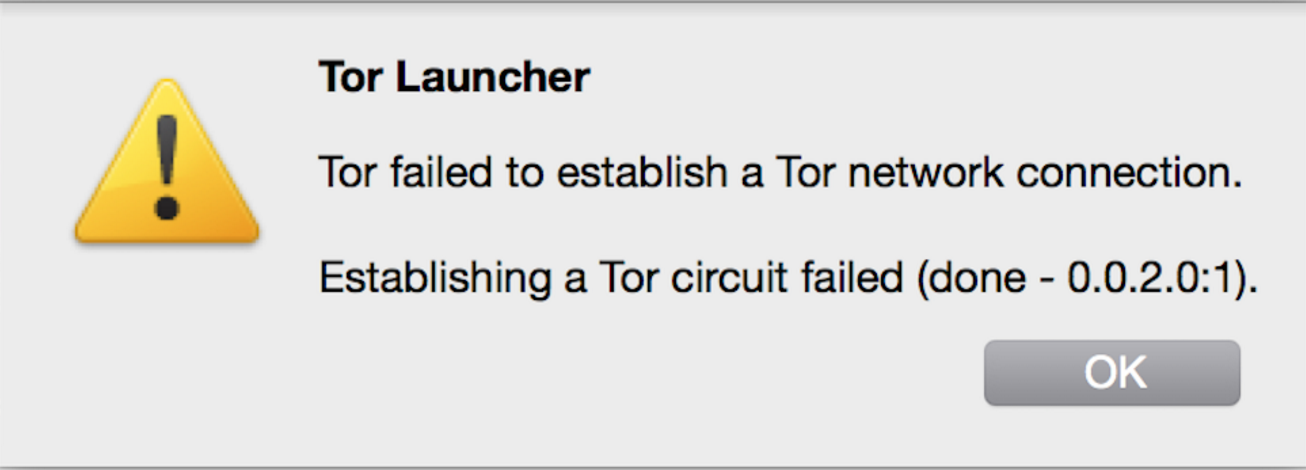
\includegraphics[width=0.5\textwidth]{error.png}
    \caption{An example of a technical error message which our participants did not understand.}
\label{fig:error}
\end{figure}

\pquote{P2}{I don't know what any of those [list of bridges] means, or what that [proxy] means at all.}
\pquote{P3}{The vocabulary is really challenging, for someone not doing IT work.}

\noindent {\bfseries Challenge 2: Users do not know if they should connect directly or configure a connection.} 
Participants incorrectly determined that a blocked torproject.org website meant that Tor relays were censored, configuring bridges and proxies when they did not need to. Other participants were not able to determine that a failed direct connection to the Tor network was the result of the Tor network being censored. \\

\noindent {\bfseries Challenge 3: Users did not know how to choose which bridge and pluggable transport.}
On the bridge configuration screen, participants were intimidated by the names of the bridge transports. The most common behavior was to configure with the recommended bridge option (obfs3). If the recommended one did not work, participants did not know how to choose another. 

\pquote{P8}{I have no clue what's the difference between flashproxy, fte, etc. I need to know why the built-in ones aren't working. And why do I need a custom bridge if there are options built in?}
\pquote{P7}{Since it (obfs3) said recommended, it helped actually, and I selected it because it was chosen. I saw the custom bridges option, but I didn't know what to enter there so I went with this (obfs3).}

\noindent {\bfseries Challenge 4: Users do not know when they are wrong.} 
Unfortunately, many mistakes did not result in error messages, bu warnings that went unnoticed.
When participants did encounter an error message, they did not understand what errors meant (Fig.~\ref{fig:error}).\\

\noindent {\bfseries Challenge 5: Users assume they are wrong when they are right.}
If users chose particular wrong configurations (i.e. a syntactically valid but nonfunctional proxy), they would be waiting for an indefinite period of time. 
\pquote{P16}{There doesn't seem to be a timeout on any of this stuff. Am I waiting long enough? It should work immediately.}

The progress bar also has a bug that causes it to update itself only when the level of progress increases.
If progress bar reaches a 90\% and fails, the next attempt will apparently have regressed to 0\% and remain there until the progress reaches >90\%. Due to this, participants assumed that their subsequent attempts were wrong, even if they were correct.
\pquote{P1}{It was hard to figure out if the progress bar wasn't moving because the connection was censored, or if it was just slow.}

\noindent {\bfseries Challenge 6: Users assume that proxy is required after a failed connection.} 
All of our participants who failed to connect (5 of 16) failed for this reason. Many mistakenly assumed that they needed a proxy upon failure, because the interface passively redirects to the proxy screen (the last screen) after failure. 

\pquote{P15}{I didn't know if this computer had any proxy information. I wasn't able to find it if it did.}

From interviewing our participants, we found that these challenges result because users are not familiar with technical or Tor-specific terms, feedback on progress or an errors were inconsistent, and the interface did not instruct users on what to do in the event of a failure. 

\section{Redesigning the Configuration Interface}
\label{redesign} 

 \begin{figure*}[t]
	\centering
		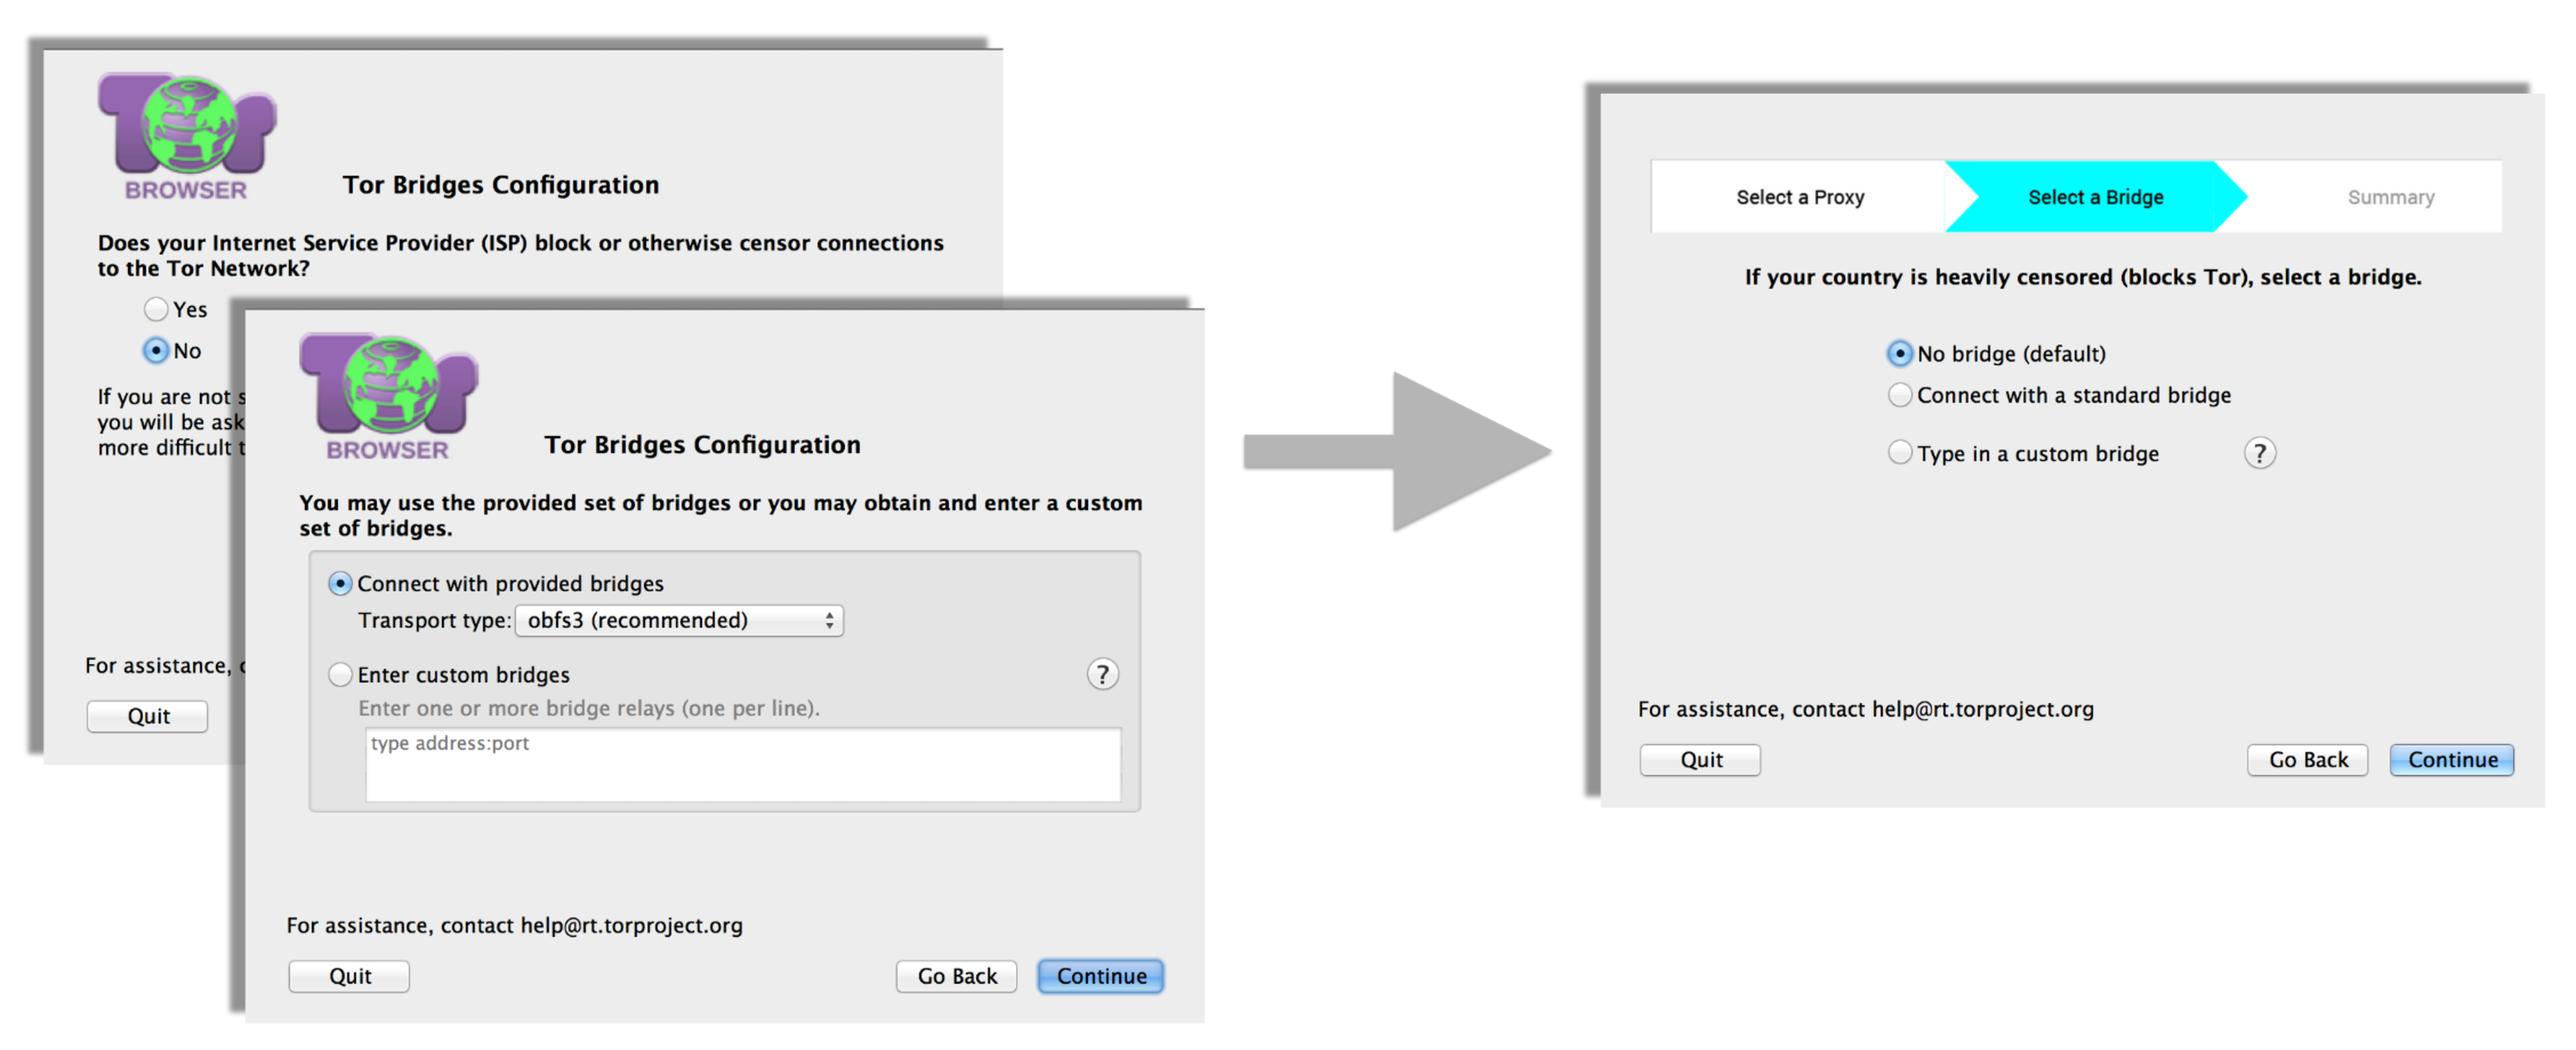
\includegraphics[width=.8\textwidth]{bridge-screens.pdf} 
		\caption{In the ``OLD'' interface, users are asked, ``Does your Internet Service Provide (ISP) block or 
		otherwise censor connections to the Tor Network?'' (B1). A ``Yes'' determines that a bridge should 
		be configured and directs to the bridge configuration screen (B2). 
		The ``NEW'' interface gives users advice on configuring bridges
		while giving the option of not configuring a bridge, on one screen (B).} 
\end{figure*} 

\begin{figure*}[t]
	\centering
		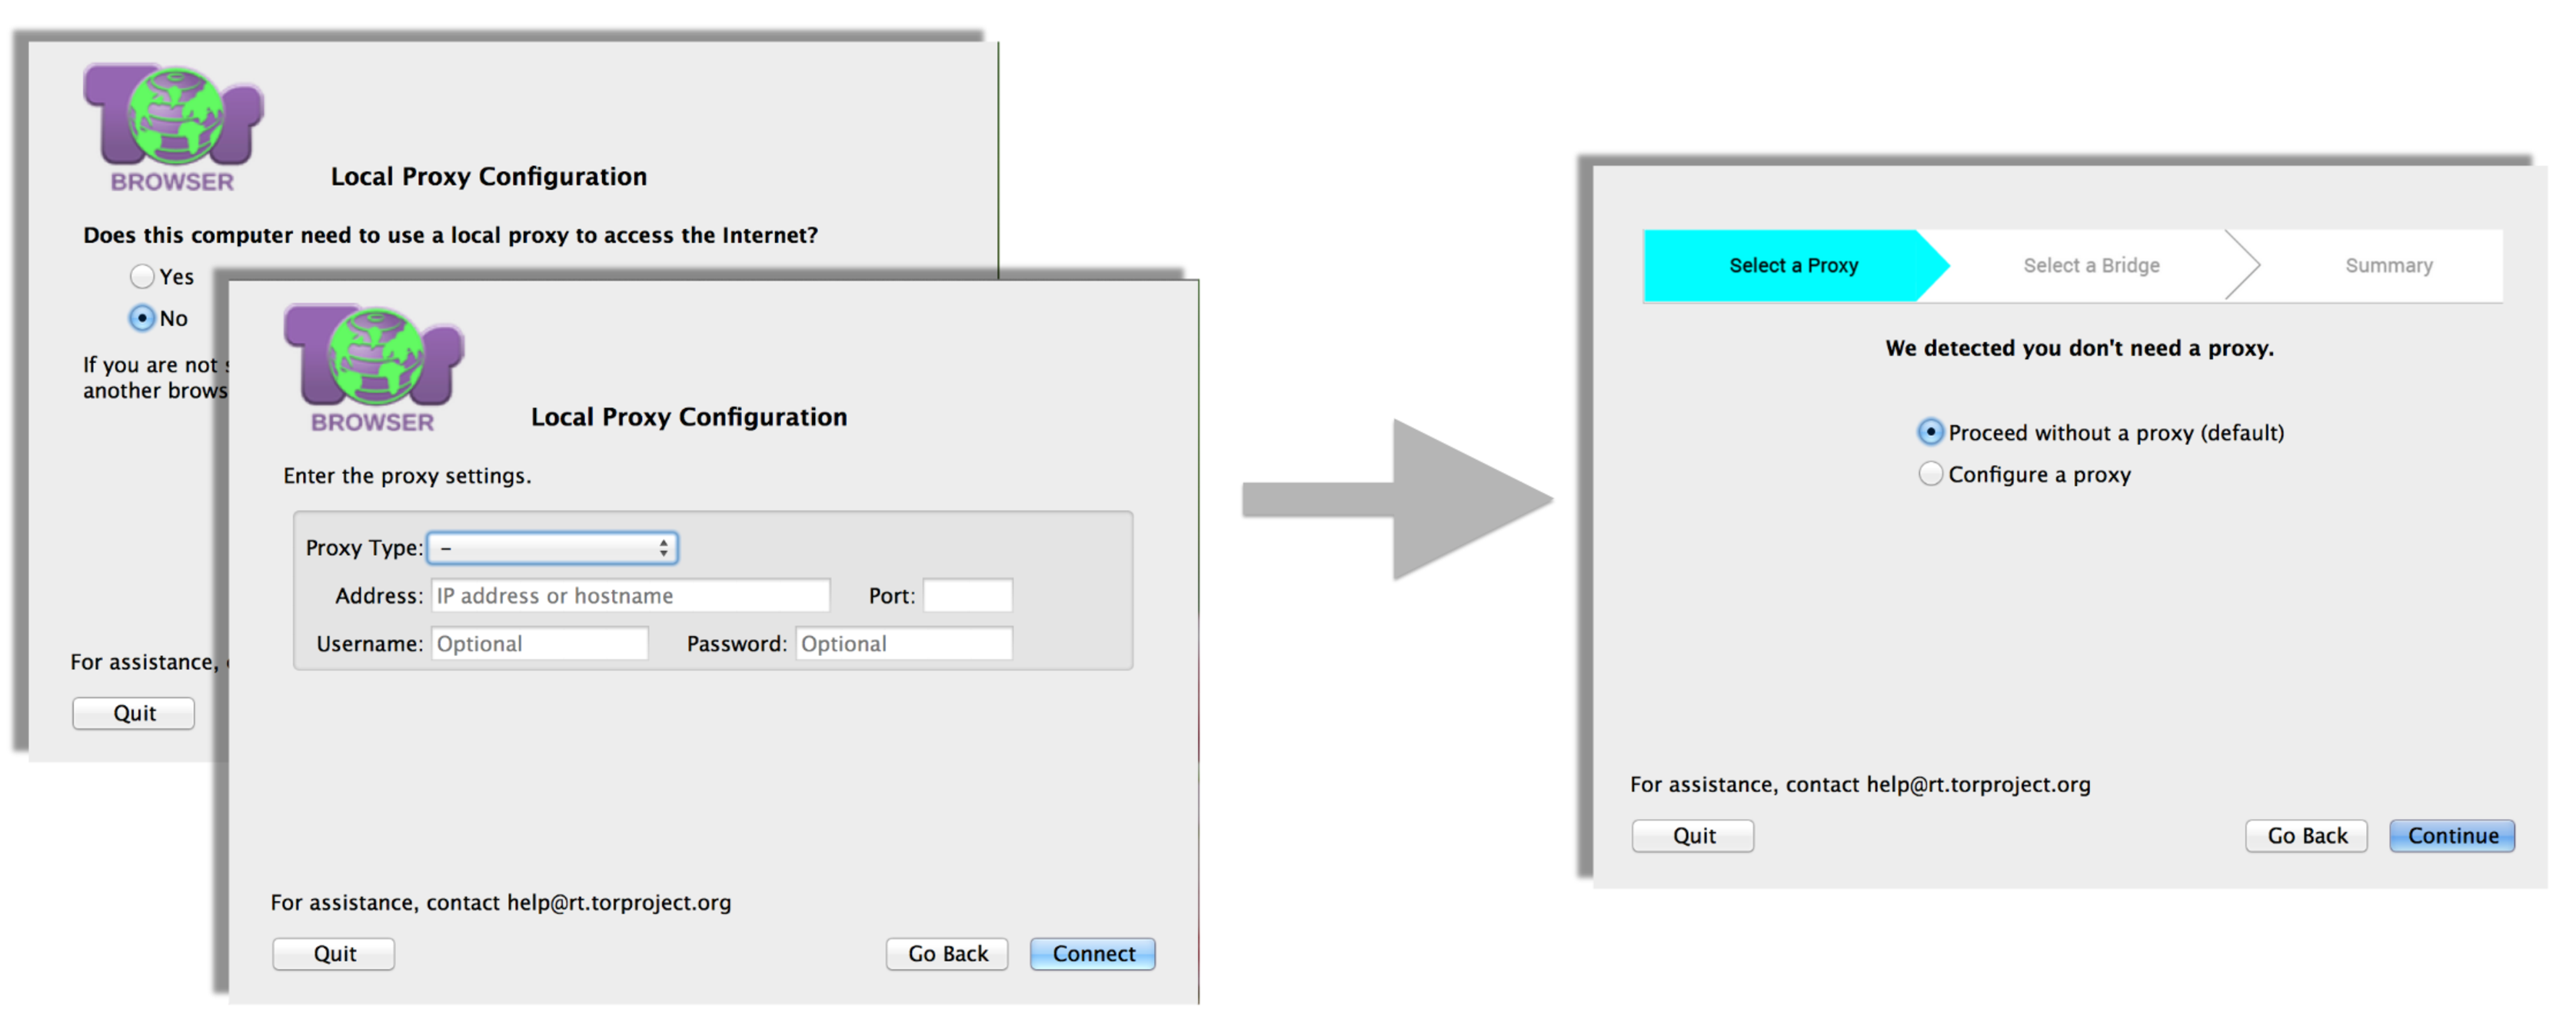
\includegraphics[width=.8\textwidth]{proxy-screens.pdf} 
		\caption{In the ``OLD'' interface, users are asked, ``Does this computer need a local proxy to connect
		to the Internet?'' (P1). A ``Yes'' determines that a proxy should be configured and directs to the 
		proxy configuration screen (P2). The ``NEW'' interface checks the local machine's proxy settings,
		and informs the user whether a proxy is required, and if so, what those settings are (P).}
\end{figure*}

From the result of our qualitative user study, we see that many users struggle with the configuration process. 
The Tor Browser configuration interface does not adequately meet our criteria from Section~\ref{sec:goals} of
managing errors gracefully, communicating in understandable language, and giving  users feedback on system state. 
We rate the severity of each issue by its frequency, impact, and persistence~\cite{nielsen1994heuristic}:\\

\begin{itemize}
\item {\bfseries Major Problem:} Error messages do not express errors in plain language nor offer solutions. 
\item {\bfseries Major Problem:} The concepts mentioned in the interface and the questions that users were required to answer were too technical for the average user. 
\item {\bfseries Minor Problem:} The configuration is not visible to the users before they attempt to connect to the Tor network or while they are connecting to the Tor network.
 \end{itemize} 
 
 \label{redesign}
\begin{figure*}[t]
\centering
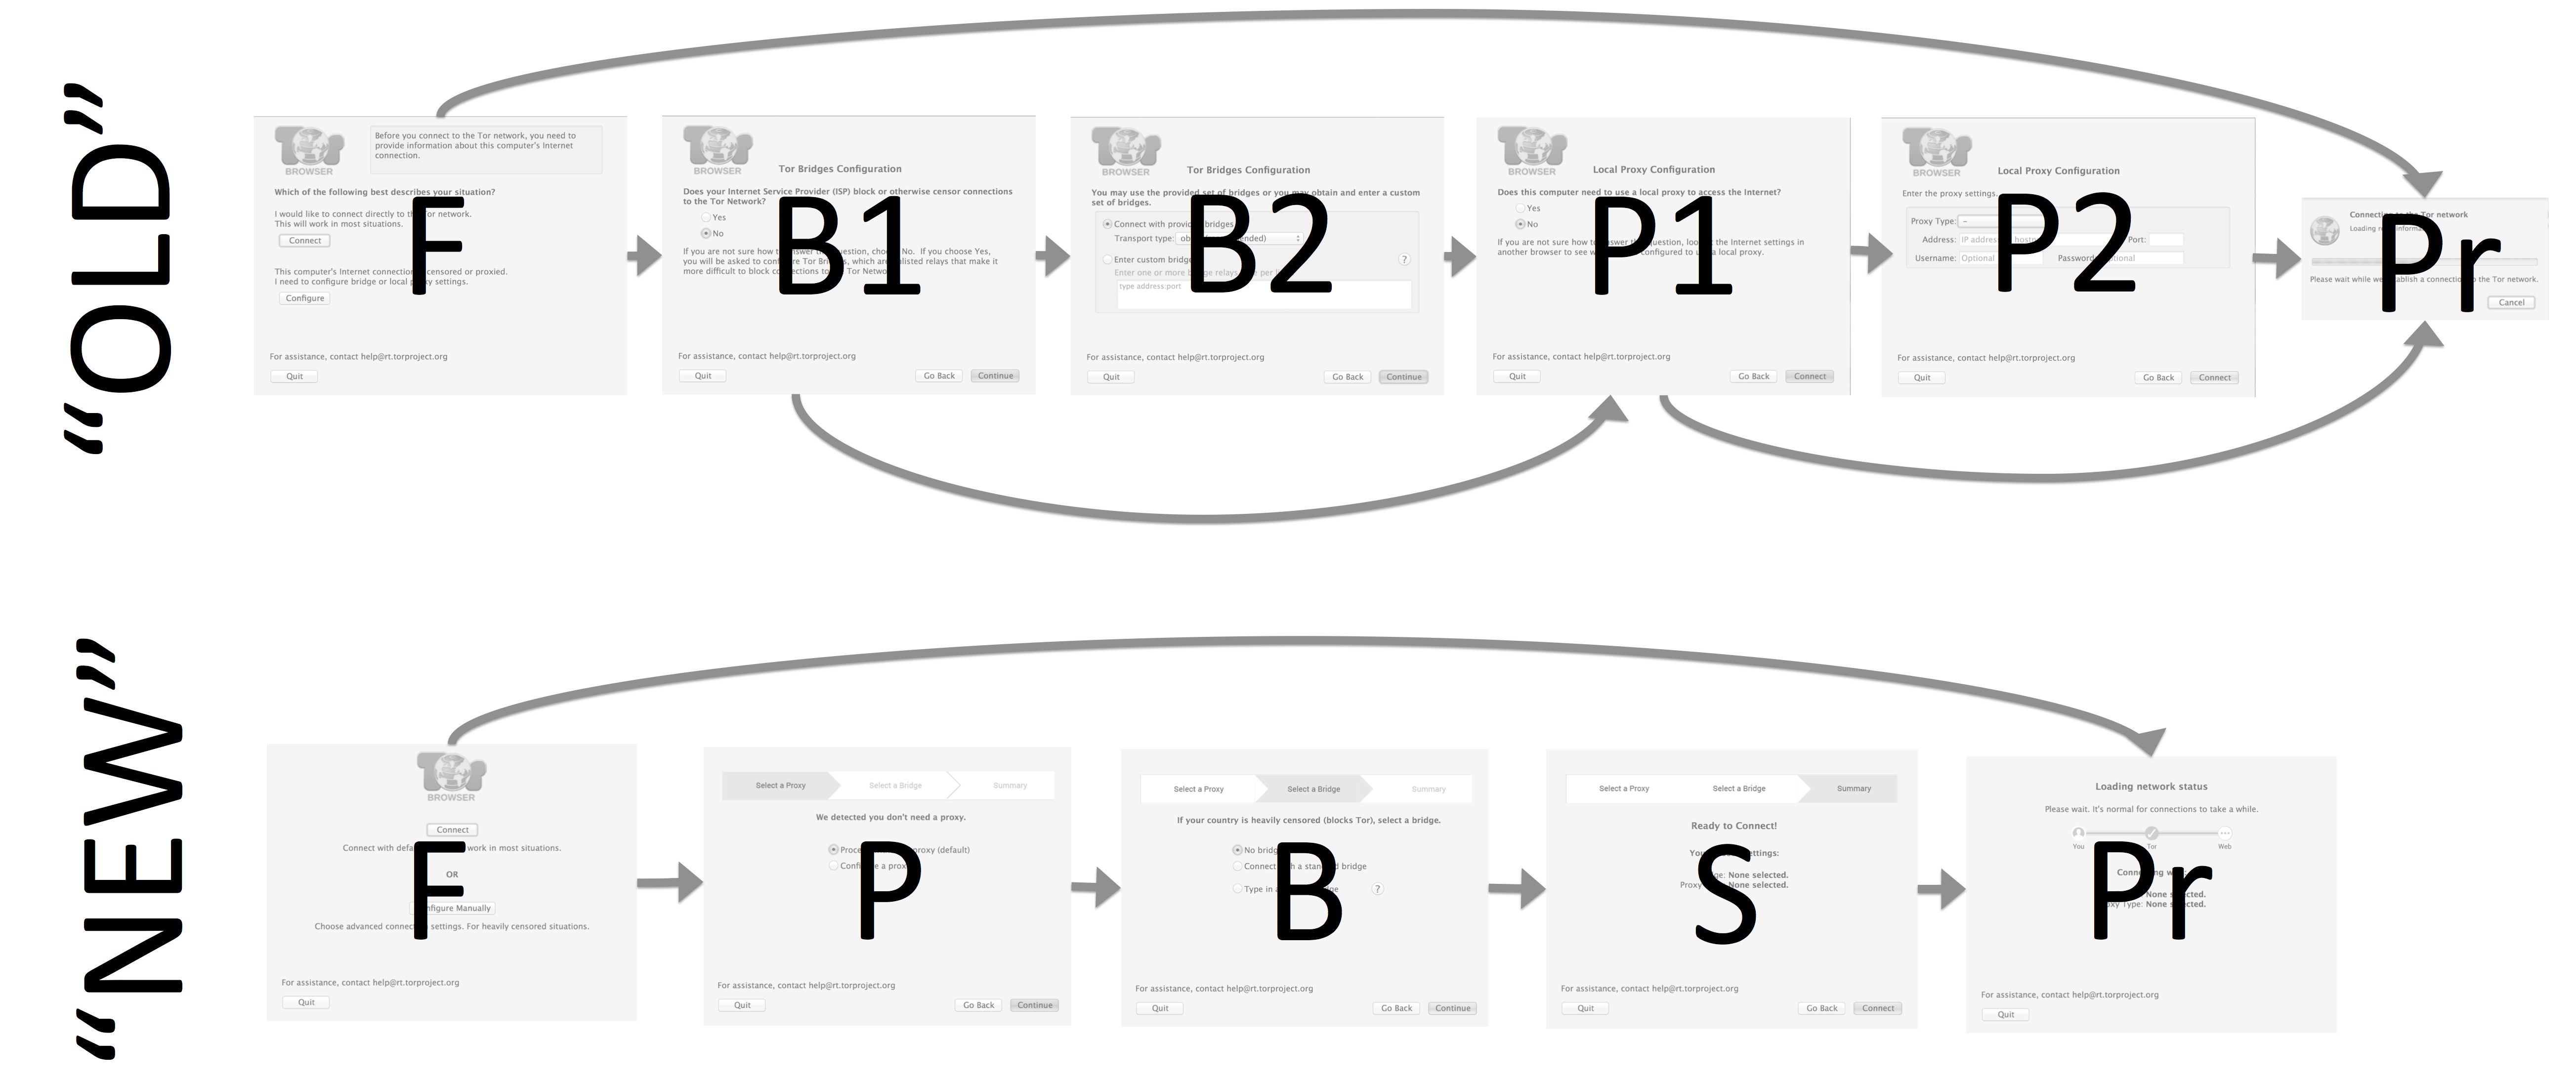
\includegraphics[width=.85\textwidth]{old-and-new-flows.png}
\caption{
Comparison of user flow in the ``OLD'' and ``NEW'' interfaces.
We collapsed the two bridge screens into one 
and also collapsed the two proxy screens into one.
We swapped the order of the bridge and proxy configuration
so it matches the order of network components (compare with Fig.~\ref{fig:topology}).
We added a summary screen as a last step before initiating a connection.\\
\textbf{F}: first screen;
\textbf{B/B1/B2}: bridge screens;
\textbf{P/P1/P2}: proxy screens;
\textbf{S}: summary screen;
\textbf{Pr}: progress bar.
}
\label{fig:flow}
\end{figure*} 

To address these three aforementioned user interaction problems, we made the following three changes to the configuration interface:  \\

\begin{enumerate}
\item {\bfseries Added instructions on what to try next on errors.} When an error occurs, text advice on what to try next is shown to the user. The advice may be to try the connection again, to choose a different bridge, or to try a connection without a proxy. 
\item {\bfseries Reduced the overall amount of text and made text less technical.} We make the text more task-centric by focusing on instructing users through the configuration process. Since users generally could not understand the technical concepts enough to influence their decisions, giving direct guidance may be a better option. 
\item {\bfseries Added system status visibility.} Before beginning any connection attempt, a summary screen displays the current bridge and proxy settings. The same information is shown on the progress screen while the connection is in progress.
\end{enumerate} 

Other changes improve empirical goals from Section~\ref{sec:goals}: task completion rate, time to completion, and safety for high-risk users. Items 5 and~6 improve task completion; 7 and~8 reduce time to completion; and 9 and~10 build users' mental models of censorship circumvention and the network components involved. Users retain full control of the configuration process.\\ 

\begin{enumerate}
\setcounter{enumi}{3}
\item {\bfseries Added guidance on choosing connect versus configure.} We labeled the configure option specifically for user in heavily censored situations, to urge users to not assume that a website censorship necessitates configuration.
\item {\bfseries Added explicit advice on choosing bridge transports.} The recommended bridge type is still obfs3. We added text that advises users to try a meek bridge if obfs3 does not work. 

\item {\bfseries Eliminated technical questions.}  We removed the gating questions that determined whether a bridge and proxy should be configured, which were highly technical and challenging for users to answer. This are two fewer screens in the revised interface. 
\item {\bfseries Added auto-detection of proxies.} In principle, the interface can guess whether a proxy is needed by scanning the operating system configuration. This purely local detection does not carry the potential risks of network probing and should be safe even for at-risk users. (In our experiment, we simulated the auto-detection by hard-coding the fact that a proxy was not required.)

\item {\bfseries Switched ordering to configure proxies first.} To build users' mental models, network components are now configured in a topologically sequential order, resembling Fig.~\ref{fig:topology} and the new progress screen. Previously, proxies were put after bridge configuration because only a small fraction of users require proxies. With auto-detection, configuring a proxy before a bridge burden users less than before.
\item {\bfseries Added clear feedback to the progress bar.} We switched the continuous progress bar to a discrete checkpoint-based progress indicator that shows the network components involved in connecting to the Tor network. This aligns with the mental model we are trying to build in the user. As connections are made with each component, the progress bar displays a green check, giving immediate feedback to the user. For instance, a user can can now see that the bridge was configured correctly, and they just need to wait to connect to the Tor network. Upon failure, users can see which components have succeeded and which have failed.
\end{enumerate}

These changes result in a redesigned interface which we refer to as ``NEW.'' Note that the new interface preserves all the functionality of the old interface and still allows users to have control over their own network traffic. 

\section{Quantitative Analyses of the Interfaces (Study 2)}
\label{sec:quantitative}
Having identified problems with the existing interface
and done a redesign in an attempt to ameliorate them,
we quantify the existing problems
and the impact of our changes with a study involving a larger number of users.
We split participants by simulated censorship environments,
and between old and new interfaces.

\subsection{Setup}
We ran our experiment at Xlab, the Experimental Social Science Laboratory at the University of 
California, Berkeley. Xlab has 36 Windows~7 laptops, separated by cubicle walls. 
Though Tor Browser runs on other operating systems,
testing was only done on Windows, as a byproduct of using Xlab. 

We augmented the interfaces with instrumentation 
to log every meaningful interaction
(button presses, menu selections, screen changes).
We wrote scripts to automatically set up the simulated censorship environment, install necessary software, 
start the video recording, and save the logs and videos.
We recorded the participants' computer screens
throughout the experiment to capture non-interface activity such as 
web searching and inspection of system networking settings.

\subsection{Recruitment}
We recruited 124 participants, about 20 for each
of the six combinations of censorship environment
and interface revision.
Data analysis considerations deem 20 participants per combination a 
minimum to assume normal distributions, and 60 participants
per interface revision is adequate to have a meaningful effect size.

We recruited half of our users from Craigslist, and half of our participants from 
the Xlab participant pool. Although Xlab participants are not limited to UC Berkeley students and staff,
a majority of the participants are from campus. For this reason, we chose to recruit 
half of our participants from Craigslist to ensure a diverse set of participants. 
The recruitment text vaguely suggests testing a piece of software, and does not require
that users provide information in advance (Appendix~\ref{quantitative-recruitment}). 
Out of our 124 participants, 59 were recruited from the Xlab pool and the other 65 were
recruited from Craigslist. Ages ranged from 18 to~68 years
($\mu = 28.9$, $\sigma = 12$). 56.8\% were male and 
84.8\% of our participants had at least a college education.

\subsection{Procedure}
The one-hour, multi-participant procedure begins when all participants are sitting at their
respective computers in Xlab. Each computer is equipped with an instrumented old or new version
of Tor Browser, Chrome, Firefox, Internet Explorer,  Chrome, and VLC (for screen recording).
Each computer was assigned one of the six conditions in the beginning of the study. Participants
were assigned to the seats at random, effectively being assigned a configuration launcher and
simulated censorship environment combination at random. 

Participants are firstly informed of the risks of the study and consenting to data collection.  At
this time, participants are given the chance to leave the laboratory if they do not consent to 
the experiment conditions. When every participant left in the room has turned in their consent
form, the experiment formally begins. A researcher informs the participants that they are in a
simulated censorship environment, instruct them to visit a sample blocked website on a 
non-Tor browser of their choice to illustrate the situation, and ask them to 
complete a worksheet that asks to visit one blocked website (Appendix~\ref{quantitative-script}). 
To mirror the qualitative study, we chose Wikipedia's featured article of the day 
as the blocked website to visit on their worksheet. 

After instructions, researchers maintained minimal interactions with the participants, 
only answering logistical questions. Participants had
about 40 minutes to complete their worksheet.
(In our analysis we defined the cutoff time to be 40 minutes and 8~seconds
in order to include a participant who finished at the wire.)
The participants do not know the details of their censorship environment,
only that they are actively being censored. Participants needed to configure Tor Browser to 
circumvent the simulated censorship. 

After users completed the browsing tasks, they took a short exit survey (Appendix~\ref{quantitative-exit-survey})
collecting their demographics. All users were instructed to sit until the end of the experiment,
regardless of when they had completed their task. After the 40 minutes were up, 
participants were officially informed that their time was up, and were given their payment of 
\$30 for their time. 

\subsection{Results} 
Out of our 124 recruited participants, 116 provided valid data. We have 58 participants who tested the new interface, and 58 who tested the old interface. 38 participants were in E1, 38 participants were in E2, and 40 participants were in E3. Since our experiment ended after 40 minutes, we chose to assign the maximum time of 40:08 minutes to participants who did not succeed. Table~\ref{table:participant-summary} summarizes the rate of success and time to success for our participants' based on their interface version and environment combination. 

\begin{table}
\centering
	% Generated by info.R.
	\begin{tabular}{l r r r r}
	& \multicolumn{2}{c}{success rate} & \multicolumn{1}{c}{median time} \\
	& \multicolumn{2}{c}{after 40 minutes} & \multicolumn{1}{c}{to success} \\
	\noalign{\hrule}
	E1-NEW & 19/19 & 100\% & 0:20 \\ % medians of only finished: 0:20 
	E1-OLD & 19/19 & 100\% & 1:01 \\ %medians of only finished: 1:01
	E2-NEW & 18/19 & 95\% & 3:32 \\ %medians of only finished: 3:22
	E2-OLD & 16/19 & 84\% & 5:00 \\ %medians of only finished: 3:13
	E3-NEW & 13/20 & 65\% & 20:56 \\ %medians of only finished: 12:38
	E3-OLD & 10/20 & 50\% & 40:08 \\ %medians of only finished: 18:16 
	\end{tabular}
\caption{
A summary of participants' success in circumventing censorship
given their simulated censorship environment and version of Tor. Those who
failed to connect successfully were assigned the maximum time of 40:08.
}
\label{table:participant-summary}
\end{table}

\subsubsection{Rate of Success} 
5 more participants with the new interface were able to successfully circumvent censorship and connect to the Tor network. Due to the limited number of participants, this difference is not large enough to rule out the possibility of random chance being the cause for the difference. However, this does suggest that users are equally likely to succeed with the new interface. 
% impact of version on success: not significant (Mann--Whitney $W = 5.5$, $p = 0.8248$)
%impact of env on success: not significant (Kruskal--Wallis $\chi^2 = 4.7059$, $\mbox{df} = 2$, $p = 0.09509$)

Table~\ref{tab:attempts-bridge-proxy} shows the configuration settings of the first successful bootstrap in each environment and interface combination. Note that only four of the default bridges were used to connect successfully for the first time. Users avoid making decisions when a recommendation is given and tend to avoid/fail with more advanced options. Participants who were in environments in which the recommended bridge (obfs3) worked did not configure another bridge, not taking advantage of the various default bridges available to them. Participants who were in environment that required a meek or custom bridge only were able to succeed with a meek bridge.

\begin{table}
\centering
% Generated by attempts.R, and manually reordered:
\begin{tabular}{r c c c c c c}
& \rotatebox{90}{E1-NEW} & \rotatebox{90}{E1-OLD} & \rotatebox{90}{E2-NEW} & \rotatebox{90}{E2-OLD} & \rotatebox{90}{E3-NEW} & \rotatebox{90}{E3-OLD} \\
no bridge, no proxy & 17 & 13 &  &  &  &  \\
obfs3, no proxy & 2 & 6 & 18 & 16 &  &  \\
meek-amazon, no proxy &  &  &  &  & 7 & 4 \\
meek-google, no proxy &  &  &  &  & 5 & 4 \\
meek-azure, no proxy &  &  &  &  & 1 & 1 \\
no bridge, 3rd-party proxy &  &  &  &  &  & 1 \\
DNF &  &  & 1 & 3 & 7 & 10 \\
\end{tabular}
\caption{
Bridge--proxy combinations that led to the first successful bootstrap
in each environment and interface.
Most E1 participants used a direct connection,
but a few tried a built-in obfs3 bridge.
All the E2 participants who succeeded,
did so with obfs3 (the recommended bridge type)---none tried
a different bridge before obfs3.
All of the successful E3 participants, but one,
used one of the meek bridges.
The remaining E3 participant succeeded in an unexpected way:
by searching the web for an open proxy and configuring it
as the proxy setting.
}
\label{tab:attempts-bridge-proxy}
\end{table}


\subsubsection{Time to Success} 
Although the median times to completion for participants of the new interface are less than those with the old interface (Table~\ref{table:participant-summary}), this difference is not statistically significant. The level of censorship had a significant impact on the time to success. The more difficult the censorship environment, the longer participants took to configure their connection (Kruskal--Wallis $\chi^2 = 80.926$, $\mbox{df} = 2$, $p < 10^{-15}$). The distribution of participants' time to success can be seen in Fig.~\ref{fig:time_to_success_clamped}.
%impact of version on time to success: not significant ($W = 1569$, $p = 0.07796$)
%impact of env on time to success : significant (Kruskal--Wallis $\chi^2 = 80.926$, $\mbox{df} = 2$, $p < 10^{-15})

\begin{figure}
\centering
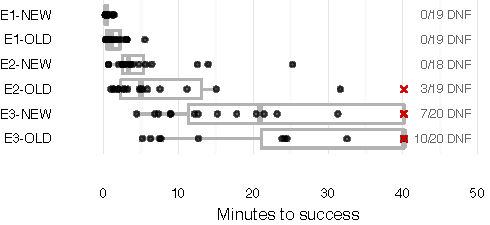
\includegraphics{time_to_success_clamped}
\caption{
Time to first success, by censorship environment and interface.
The dots show the raw completion times,
while the boxplots show the medians and interquartile ranges.
The ``DNF'' figures at the right show the number of participants 
who did not finish in the time allotted.
Here, non-finishing participants are assigned the maximum time of 40:08
for the purpose of computing the median.
}
\label{fig:time_to_success_clamped}
\end{figure}

In our experiment, participants had 40 minutes to circumvent censorship. Fig.~\ref{fig:time_to_success_ecdf} shows the cumulative success rates over time. Participants were less and less likely to succeed as time went on. Users in the wild will likely not be motivated to configure their connection for 40 minutes. Table~\ref{table:less_time} shows that if users were only willing to put in a minute or so of their time, users in intermediate and heavily censored environments will be unable to connect. Even if users were willing to dedicate 10 minutes to configuring their connection, most users in heavily censored environments will be unable to connect. Ideally, users should be able to connect to Tor within a couple of minutes, regardless of their censorship environment. We propose ideas on how to achieve this in section~\ref{recommendations}. 

\begin{figure}
\centering
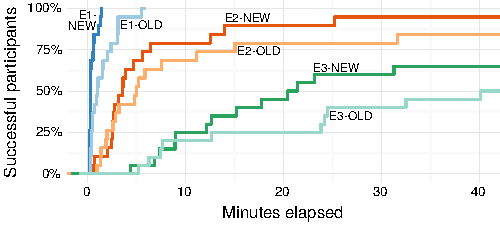
\includegraphics{time_to_success_ecdf}
\caption{
Cumulative success rates over time, by censorship environment and interface.
We stopped participants after 40 minutes. Here, those who did not finish were assigned
an arbitrarily high number greater than 40 minutes for the purposes of plotting. 
}
\label{fig:time_to_success_ecdf}
\end{figure}

\begin{table}
\centering 
	% Generated by info.R:
	\begin{tabular}{l r r r r}
	& \multicolumn{1}{c}{1.5~m} & \multicolumn{1}{c}{10~m} & \multicolumn{1}{c}{20~m} & \multicolumn{1}{c}{40~m} \\
	\noalign{\hrule}
	E1-NEW & 100\% & 100\% & 100\% & 100\% \\
	E1-OLD & 58\% & 100\% & 100\% & 100\% \\
	E2-NEW & 11\% & 79\% & 89\% & 95\% \\
	E2-OLD & 16\% & 68\% & 79\% & 84\% \\
	E3-NEW & 0\% & 25\% & 45\% & 65\% \\
	E3-OLD & 0\% & 20\% & 25\% & 50\% \\
	\end{tabular}
\caption{This Table shows what the success rate would have been
at different cutoff times.
For example, every E1-NEW participant finished within 90 seconds,
but only 58\% of E1-OLD had finished by that time.
After 10 minutes, 79\% of E2-NEW and 68\% of E2-OLD had finished.
After 20 minutes, 45\% of E3-NEW and only 25\% of E3-OLD had finished.}
\label{table:less_time}
\end{table}

\subsubsection{Active Configuration Time} 
We summarize each participant's actions throughout the experiment in Fig.~\ref{fig:all-participant-edges}. Each row in Fig.~\ref{fig:all-participant-edges} corresponds to a participant in our experiment. The bar represents a participants' path through the interface, illustrating time spent on each screen, transitions between screens, how many attempts were made, and if they were eventually successful. 

\begin{figure*}
\centering
% This is a manually edited version of the automatically generated
% all-participant-edges graphic. It is edited to have better scale labels for
% the treatments.
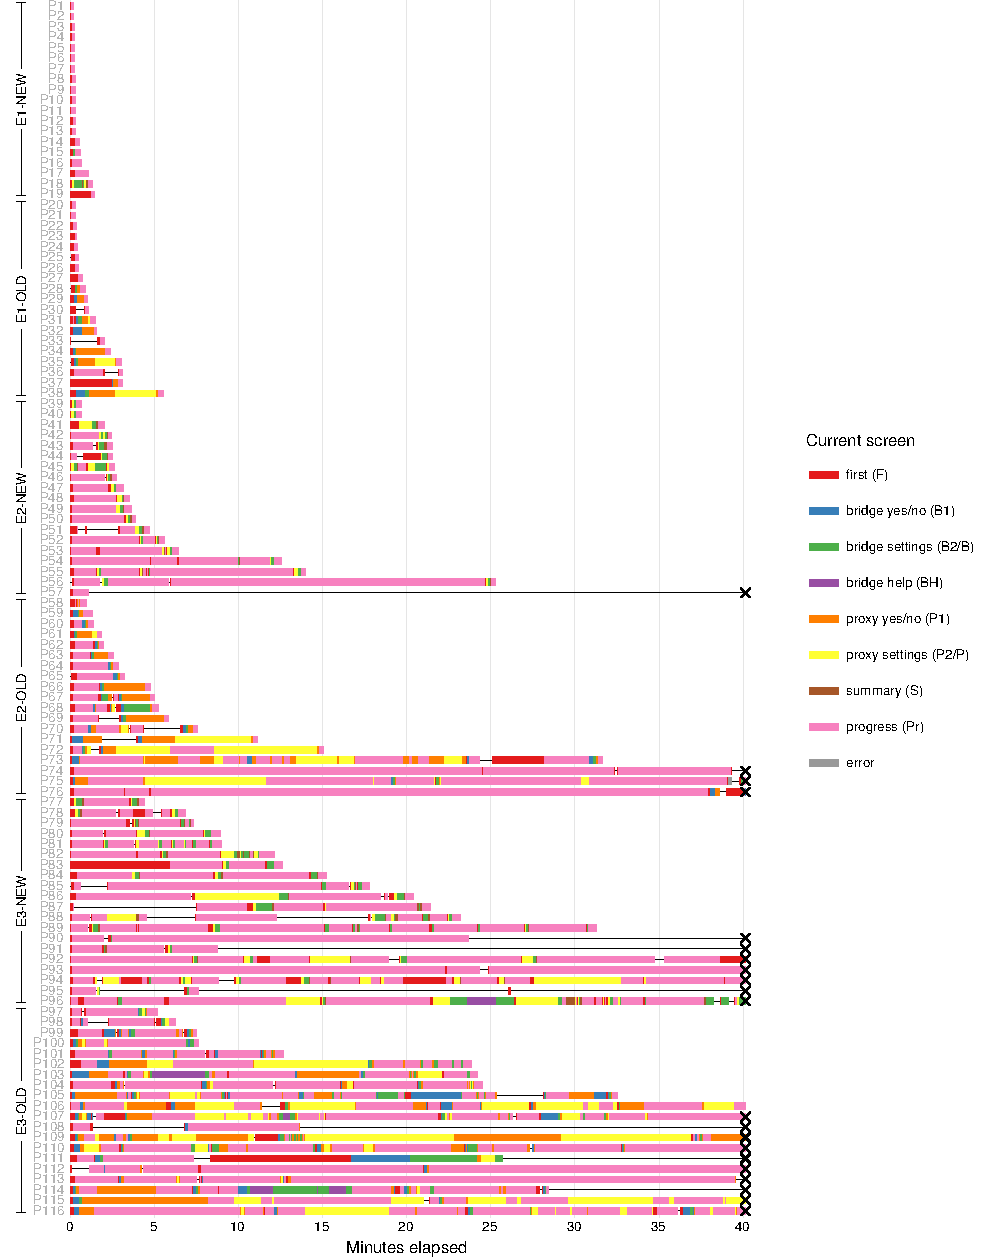
\includegraphics{all-participant-edges-scales}
\caption{
Summary of participants' actions throughout the entire experiment.
Different colors indicate which screen was shown at each moment.
The narrow black lines show the times when the configuration interface
was not running; i.e., a participant was doing something else
such as searching the web in another browser.
The overall length of the lines show the total time to completion,
except for those we cut off after approximately 40 minutes.
}
\label{fig:all-participant-edges}
\end{figure*}

While we did not find a statistically significant difference between the overall time to success between the old and new versions of the interface, the time to success was largely dominated by the time spent waiting to connect to Tor, rather than actively configuring the interface. Table ~\ref{table:overall_time} shows the time spent on each screen while participants used the interface, which shows that participants spent 57\% of their overall time at the progress screen. Participants using the new interface and old interface waited spent approximately the same amount of time overall on the progress screen (359 minutes versus 339 minutes), which accounts for 78\% and 45\% of their overall time, respectively. We attribute this to a combination of instructions that tell the user to ``wait a couple minutes'' because connections usually take a while to bootstrap and the lack of timeout on the progress screen which keeps the users waiting indefinitely, which were present in both versions of the interface. 

\begin{table}
\centering
	\begin{tabular}{c r r r r r}
	 & First & Proxy & Bridge & Summary & Progress \\
	\noalign{\hrule}
	All &  10\% & 24\% & 8\% & 1\% & 57\% \\
	NEW & 9\% & 7\% & 4\% & 2\% &  78\% \\
	OLD & 10\% & 35\% & 11\% & 0\% & 45\% \\
	E1 & 33\% & 16\% & 23\% & 1\% & 27\% \\
	E2 & 11\% & 18\% & 8\% & 1\% & 63\% \\
	E3 & 8\% & 27\% & 8\% & 1\% & 57\% \\
	\end{tabular}
\caption{overall time} 
\label{table:overall_time}
\end{table}

Perhaps a more meaningful measurement of time is the amount of time participants actively spent configuring their connection. We define this as the amount of time that participants spent on the interface, except for time spent on the progress screen. This is a simplified notion active configuration time, since some participants searched for help on the web while they were waiting. However, this behavior was equally likely in the new and old interface conditions.

The new interface results a statistically significant reduction in the overall active configuration time (Mann--Whitney $Z = -3.055$, $p = 0.00225$, $\mbox{effect size} = 0.284$), while maintaining the same probability for success for the user. We believe that getting rid of the technical bridge and proxy questions, instructing participants that they did not need a proxy, and simplifying the interface attributed to the reduction in time. 
%The impact of the environment on active time is significant (Kruskal--Wallis $\chi^2 = 51.978$, $\mbox{df} = 2$, $p = 10^{-11}$)

\subsection{Discussion} 
This section talks about general trends in user behavior, common failure cases, and our recommendations for 
improving the Tor configuration interface. 

\subsubsection{Observations}
These are general observations made from our data set of participants, which may have biases.\\

\begin{description}
%connect vs configure
\item {\bfseries Users try the easy path first.} Users still do not seem to know how to differentiate between censored websites and censored Tor relays, and just try the easy option to connect directly to the Tor network first, leaking that they are connecting to Tor on the network.  81\% (94 of 116) of first attempts were to connect directly, 86\% (50 of 116) from the new interface and 76\% (44 of 116) from the old interface. 

% impacts of making the proxy page ``automated'' 
\item {\bfseries Users wasted time configuring proxies.} Users believed that they needed proxies to connect. This confusion prevented users from configuring their bridges correctly. Participants with the new interface who were explicitly told that they did not need a proxy spent 31\% of their active time configuring proxies and participants in the old interface who did not receive feedback spent 63\%.

% impacts of giving people advice on which transport to choose.
\item {\bfseries Certain transports were chosen with high probability.}
Of those who tried an obfs3 bridge and failed, 
66\% (10 of 15) participants with the new interface and 38\% (5 of 13) participants with the old interface chose meek as their second bridge. We suspect that flashproxy was a popular choice, because it is listed first in the drop-down menu. Many bridges listed at the end of the drop-down menu were not chosen. 

%error messages
\item {\bfseries There were (almost) no error messages.} Many waited for minutes at the progress screen, but never saw an error message. There were warnings, but those warnings went largely unnoticed by our participants. Across both versions of the interface, only one participant ever saw an error message. 

% progress bar
\item {\bfseries People waited a long, long time at the progress bar.}
Participants spend so much time waiting. Some are dutifully following the directions to wait, while others are lost for what to do and choose to wait in frustration.   
\end{description} 

We are unable to state the efficacy of our attempts to make instructive and understandable error messages due to lack of data. Users in the new interface were more likely to chose meek bridges, but we cannot say if this can be attributed to the advice we added on the bridge configuration screen to choose a meek bridge after an obfs3 bridge fails. It is unclear why users with the new interface chose to configure proxies after explicitly being told that they do not need one. 

\subsubsection{Reasons for Failure} 
Failure is common. 64\% (74 of 116) of first attempts to connect failed and 79\% (376 of 462) of total attempts to connect failed. 20\% (22 of 116) of participants failed entirely. Reasons for failure were determined by a combination of log processing (i.e., how much time was spent on a particular screen) and video observation (i.e., observing what they searched for online). \\ 

\begin{description}
\item {\bfseries Only connected directly. (8/23)} These participants tried a direct connection. When that failed, they tried the same configuration, over and over, without trying other configurations, no matter how many times they failed. It was common to restart the interface, check Internet settings, and wait between subsequent attempts. 
\item {\bfseries Did not know what to do next. (6/23)} After a failed direct connection and a failed default obfs3 bridge connection, these participants did not know what to do next. They often tried those configurations again or gave up. 
\item {\bfseries Thought that they needed a proxy (5/23)} After a couple failed attempts, these participants assumed that they needed a proxy. They spent the time trying to configure a proxy, usually without trying other bridges. 
\item {\bfseries Used the bridges auto-responder incorrectly (3/23)} Three participants in our heavy censorship environment figured that the recommended bridge and most hard-coded bridges were not working and found the auto-responder through the help button. However, they all failed to get a response. For details, see Appendix~\ref{failed-participants}.
\end{description} 

We discarded data on participants who chose to download their own version of Tor Browser online. Some downloaded their own version without trying the provided one on their desktop, while others did so after feeling frustrated with the provided version. Appendix~\ref{tor-downloads} gives the unfortunate details of where Tor was downloaded when torproject.org was blocked.

\subsubsection{Recommendations}
\label{recommendations}
Based on our observations of general behavioral trends and common failure cases, we make the following recommendations to increase success rate and decrease overall time spent in the interface: \\

\begin{description}
\item {\bfseries Automate configuration after failure.} After one unsuccessful attempt, the user has already indicated to their censor that they are connecting to Tor. Automating the configuration process thereafter will have no increase in risk, bu can help a majority of users. 64\% of participants who failed their first attempt. Users in more difficult censorship environments are more likely to benefit from this, as 5\% of participants in the mild censorship environment, 84\% participants in intermediate censorship environment, and 100\% of participants in the heavy censorship environment failed the first time.
\item{\bfseries Hide infrequently used options.} Informing users that they did not need a proxy was not enough to deter users from spending time on configuring a proxy. Only a small fraction of the Internet population requires a proxy to connect to the Internet. Hiding the proxy screen by default and only showing it after it has been detected as necessary can focus user efforts on configuring bridges.
\item {\bfseries Be explicit about recommendations.} Being explicit about the order in which a user should choose bridges will result in higher rates of success and lessen cognitive load on the user. Most participants followed recommendations about which bridge to choose, and many did not know what to do after the recommended bridge failed. 
\item{\bfseries Set a timeout on the progress bar.} Informing users that they have failed earlier will decrease the overall time to success, create an opportunity to give suggestions, and reduce user frustration. 
\item{\bfseries Have a user-tolerant auto-responder.} Having the auto-responder default respond with bridges or catching common errors (such as typing ``get bridges'' in the subject line) can help those who need custom bridges. 
\end{description} 

We also encourage best practices, such as providing a summary screen to let the user know the configuration settings before connecting, having a checklist progress bar to give users feedback on what network component needs configuring, and rewriting screen text and error messages to be more instructive and understandable. 

\section{Limitations} 
The interface was only tested on Windows machines, which were the only types of machines in Xlab. The configuration interface uses the native operating system's elements and their respective styling, so an interface looks slightly different across different operating systems. Participants who are not accustomed to using Windows machines may have been slower than usual to complete the given task, but this effect should affect all of our conditions equally. 

Our study was conducted in an inorganic setting, which can cause our participants to be under or over-motivated. Our participants had a monetary incentive to connect to Tor, whereas a real user in a censored environment would want to reach a particular website or service. The nature of the experiment places social pressure to attempt connect for the whole duration of the session, whereas participants may have given up earlier if they were not in an organic setting.   

We did not test cases in which the user is required to configure a custom bridge or proxy. Our participants were from one geographic location in the United States and were able to speak English.

\section{Future Work} 
Throughout the qualitative user study, redesign of the interface, and the quantitative user study, we collaborated and communicated with Tor developers. Redesigning the configuration interface was a mutual interest. In fact, Tor version~4.5 incorporated textual and navigational changes based on our redesigned interface. We plan to work with Tor developers to integrate helpful changes. This process will entail debugging our code, merging changes with the current version of Tor, making high-fidelity graphics that align with style guides, and finalizing the advice to give to users in the interface. 

We took an approach that optimized for the average case user manually configuring a connection. Additional user studies that focus specifically on users in heavily censored environments, or increasing the amount of automation in the configuration process can yield to higher rates of success and faster time to success. We encourage future work to explore some of the non-conservative changes and alternate approaches that we were not able to test in these series of experiments.\\

\begin{description}
\item{\bfseries Automate the configuration.} Complete automation and network probing sounds like a radical idea, but this would not harm users today (as far as we know). Most users would leak that they are using Tor when trying to circumvent an advanced censor, since most first attempts to connect fail. 
\item{\bfseries Ask about the risk.} Ask the users if they would be at risk if the process was automated, and automate the configuration process for all who are not at risk. The ones at risk will configure manually. The complication with this approach is that users may not be qualified to answer this question or may not trust Tor to answer honestly. 
\item{\bfseries Ask if users if they know what to do.} We ask users if they know how to configure a bridge and proxy, and automate the configuration process if they do not. However, there are ethical implications of making mistakes on behalf of the users if there is risk involved. 
\end{description}

We believe that automation, risk, and identifying struggling users are all integral to making significant improvements to the configuration process. 

%\section {Acknowledgments}
%{\color {red} Rowilma del Castillo for setting up Xlab, Nima Fatemi, Isabela Bagueros, Georg Koppen, and the UX team for giving feedback, and Cecile Basnage for reviewing the UI of circumvention tools.} 
%{\color {red} Tor Browser devs for taking our recommendations to heart and implementing changes.}

\section{Conclusion} 
We conducted a series of experiments to improve the Tor Browser 5.0.3 configuration interface, which helps users circumvent censorship using Tor. The qualitative user study interviews 16 pre-screened participants about their experience trying to circumvent mild, intermediate, and heavy censorship with the current interface, giving insight into common challenges in configuring a connection, such as confusing the necessity of bridges and proxies, assuming that a correct configuration was wrong due to a progress bar bug, and not knowing what to do on failure. This feedback is used to guide the redesign of the configuration interface. 

We test the impact of our changes on 124 participants in the quantitative user study to find that that the changes made cause a statistically significant reduction in the time participants spent configuring their connection, with no decrease in success rates. We observe and quantify common behavioral trends based on logs and video recordings of our participants, and offer recommendations that we believe will greatly increase the success rate and time to success for future users. 

\bibliographystyle{abbrv}
\bibliography{pets2017-paper}

\appendix
\section{Participant Worksheet Text} 
\label{participant-worksheet}
Imagine you live in an oppressive country that censors part of the Internet. We have simulated this in the laboratory by blocking certain websites and services. The purpose of this experiment is to evaluate the use of Tor browser, which is a browser that can circumvent censorship and let you visit blocked websites. For instance, www.torproject.org is blocked. Check this by going to the site on a standard browser, like Firefox, Chrome, or Internet Explorer. It will fail to load, when you can visit other sites.

To complete this worksheet, you will need to set up Tor browser (on your desktop) correctly and use it to get to blocked site. If you can visit wikipedia, then you know that you have successfully circumvented censorship.

\section{Qualitative User Study Recruitment Posting} 
\label{qualitative-recruitment}
We are recruiting participants for an in-person research study at the University of California, Berkeley. You will need to come in to our lab and perform tasks on a computer for an hour or less. You will be compensated \$30 for participating. 
No special knowledge and no technical experience is required. If you are interested, fill out the survey at \textit{<survey link>}. 

\section{Qualitative User Study Prescreening Survey} 
\label{qualitative-prescreening}
We are recruiting participants for an in-person research study at the University of California, Berkeley. You will need to come in to our lab and perform tasks on a computer for an hour or less. You will be compensated \$30 for participating. No special knowledge and no technical experience is required.\\

\begin{enumerate}
\item{Please select when you are available. We will assign you an hour experiment time slot during one of those times.}
\item{I am able to provide my own transportation to the University of California, Berkeley campus.}
\item{Thank you for your interest! Please provide an email address where we can contact you to share more logistical details.}
\item{we are looking for a very small number of participants, so unfortunately, we may not be able to accommodate everyone who applies. Would you like us to let you know about future opportunities?}
\item{What is your gender?}
\item{What is your age?}
\item{Please select your highest completed (or current) level of education.}
\item{What is your occupation?} 
\item{Do you speak any languages other than English fluently?}
\item{If you have a personal computer, what kind do you use?}
\item{Which of the following terms have you heard of? \textit{<answer choices: a checkboxlist of the the following terms: malware, proxy services, phishing, SSL, X.511 certificates, Tor>}}
\item{How often do you use the following software or features? \textit{<answer choices: a grid of radio buttons. Software/features (rows): HTTPS on web pages, proxies or other censorship circumvention tools, virtual private networks (VPN), file or whole-disk encryption, anonymity systems (e.g., Tor), email encryption (e.g., PGP), chat or instant messaging encryption, voice communication encryption. Frequency (columns): never, less than once a month, a few times a month, several times a week, daily.>}}
\end{enumerate}
Thank you for filling out this form. You are now done!

\section{Qualitative User Study Introduction Script} 
\label{qualitative-script} 
Imagine you live in an oppressive country that censors part of the Internet. We have simulated this in the laboratory by blocking certain websites and services.  The purpose of this experiment is to evaluate the use of Tor browser, which is a browser that can circumvent censorship and let you visit blocked websites. Currently, torproject is blocked (you can check this by going to torproject.org on a standard browser, like Firefox, Chrome, or Internet Explorer). 

To circumvent censorship successfully, you will need to set up Tor browser correctly and use it to get to Wikipedia. If you are able to reach the website, then you know that you have successfully circumvented censorship. Fill out the question on the worksheet. This isn't intended to be hard, just write what you see. We want to just check you saw the website. 

Before you start, do you have any questions about what you are asked to do? 

\section{Post-Experiment Standard Interview Questions}
We asked our participants these questions after they were given time to configure Tor Browser. \\

\begin{enumerate}
\item{Can you talk us through what you did along with what you were thinking at the time?}
\item{What was most challenging part of connecting?}
\item{Were there any unfamiliar terms?}
\item{How did you decide which options to choose?}
\item{What did you think about using Tor?}
\item{What is one change you would recommend?} 
\item{Did you need any additional information?} 
\end{enumerate}  

In addition to these questions, we asked our participants about specific questions based on their observation, usually regarding a specific choice in action, a particular screen they seemed stuck on, and any errors they encountered during the configuration process. 

\section{Quantitative User Recruitment Posting}
\label{quantitative-recruitment}
We are recruiting up to 40 participants for a user study at UC Berkeley. The experiment will involve basic Internet browsing tasks. You are not eligible if you have participated in our previous sessions.\\

\indent Payment: \$30 Amazon gift card\\
\indent Duration: 1 hour \\
\indent Where: Xlab at Hearst Memorial Gymnasium\\

\textit{<list of sessions>}\\

To be eligible, you must be an adult (18 or older). This is to comply with university policies on research. 

If you are interested: 1. Email lnl@berkeley.edu with the sessions you are able to attend. We will confirm your participation and assign you a session. 2. Come to Xlab at the appointed time for the experiment.

\section{Quantitative User Study Introduction Script} 
\label{quantitative-script} 
Imagine you live in an oppressive country that censors part of the Internet. We have simulated this in the laboratory by blocking certain websites and services.  The purpose of this experiment is to evaluate the use of Tor browser, which is a browser that can circumvent censorship and let you visit blocked websites. Currently, torproject is blocked (you can check this by going to torproject.org on a standard browser, like Firefox, Chrome, or Internet Explorer). 

To circumvent censorship successfully, you will need to set up Tor browser correctly and use it to get to Wikipedia. Tor is already installed for you. On the desktop, you should see a globe icon that says ``Start Tor Browser.'' If you are able to reach the website, then you know that you have successfully circumvented censorship. Fill out the question on the worksheet. This isn't intended to be hard, just write what you see. We want to just check you saw the website. 

Afterward, we ask you to take a short survey to collect some information about you. The link is also on your worksheet.
We will give you time to complete this task. If you finish early, we ask that you sit at your desk until the remainder of the hour. Since we are recording your screen, we ask that you don't do anything personal afterward, like checking your email.

Before you start, do you have any questions about what you are asked to do? 

\section{Quantitative User Study Exit Survey} 
\label{quantitative-exit-survey}
We'd like to know more about you.  All of your answers will be stored separately from any identifying information in order to protect your confidentiality.

This survey is part of a research project being conducted by the University of California, Berkeley. If you have any questions about your rights or treatment as a research participant in this study, please contact the University of California at Berkeley's Committee for Protection of Human Subjects at 510-642-7461, or email subjects@berkeley.edu. If you agree to participate, please click Next below.\\

\begin{enumerate}
\item{What is your participant ID? (This can be found on the sticker on the left hand corner of the desk you are currently sitting at.)}
\item{What is your gender?}
\item{What is your age?}
\item{Please select your highest completed (or current) level of education}.
\item{What is your current occupation?}  
\end{enumerate}

Thank you for participating in our experiment. You are now done! Please sit at your desk for the remainder of the experiment. Our researchers will formally announce the end of the experiment. 

\section{Failed Participants} 
\label{failed-participants}

Only tried to connect directly (8/23): 
\begin{itemize}
\item E2-NEW-X21-20160323-1400
\item E2-OLD-X04-20160330-1800
\item E2-OLD-X10-20160331-1600
\item E3-NEW-X05-20160324-1400
\item E3-NEW-X17-20160323-1400
\item E3-OLD-X06-20160328-1400
\item E3-OLD-X06-20160330-1600
\item E3-OLD-X12-20160330-1800
\end{itemize} 

Did not know what to do next (6/23): 
\begin{itemize}
\item E3-NEW-X11-20160330-1600
\item E3-NEW-X11-20160331-1800
\item E3-NEW-X23-20160323-1400
\item E3-OLD-X06-20160331-1800
\item E3-OLD-X12-20160331-1600
\item E3-OLD-X30-20160328-1400
\end{itemize} 

Thought that they needed a proxy (5/23): 
\begin{itemize}
\item E2-OLD-X10-20160328-1400
\item E3-NEW-X17-20160328-1600
\item E3-OLD-X06-20160325-1800
\item E3-OLD-X06-20160330-1800
\item E3-OLD-X24-20160328-1600
\end{itemize} 

Used the bridges auto-responder incorrectly (3/23): 
\begin{itemize}
\item E3-NEW-X23-20160328-1600 (Fig.~\ref{autoresponder1})
\item E3-OLD-X12-20160325-1400 (Fig.~\ref{autoresponder2})
\item E3-OLD-X24-20160328-1400 (Fig.~\ref{autoresponder3})
\end{itemize}   

\begin{figure}[h]
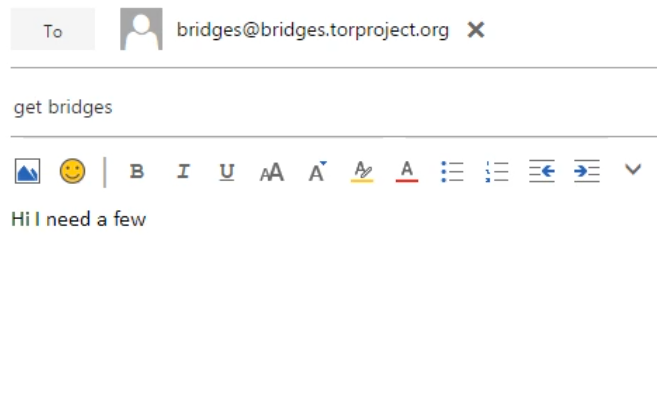
\includegraphics[width=0.5\textwidth]{../experiment/processing/failed-participants/20160325-140813-bridgeresponder-redacted.png}
\caption{The message that E3-NEW-X23-20160328-1600 attempted to send to the bridge auto-responder. The message was sent to the wrong address: bridges@bridges.torproject.org instead of bridges@torproject.org.}
\label{autoresponder1}
\end{figure} 

\begin{figure}[h]
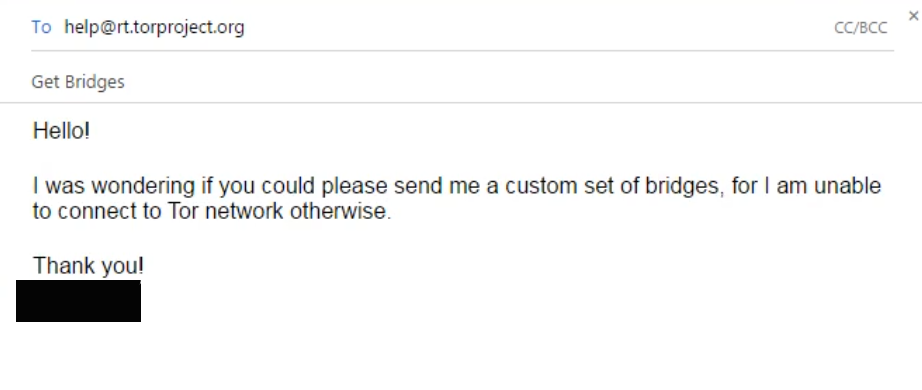
\includegraphics[width=0.5\textwidth]{../experiment/processing/failed-participants/20160328-133857-bridgeresponder-redacted.png}
\caption{The message that E3-OLD-X12-20160325-1400 accidentally sent to the helpdesk rather than the bridge auto-responder. The participant should have used the address bridges@torproject.org, not help@rt.torproject.org. Since the helpdesk address is not an auto-responder, there was no reply.}
\label{autoresponder2}
\end{figure} 

\begin{figure}[h]
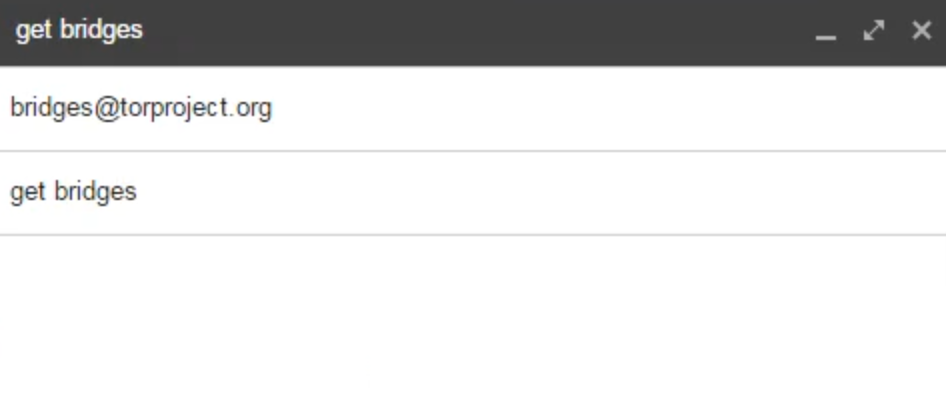
\includegraphics[width=0.5\textwidth]{../experiment/processing/failed-participants/20160328-155924-bridgeresponder.png}
\caption{The message that E3-OLD-X24-20160328-1400 sent to the bridge auto-responder. A correct message is a ``get bridges'' in the body of the message, with any non-empty subject. Since this request was incorrectly formatted, there was no reply.}
\label{autoresponder3}
\end{figure} 

\section{Tor Downloads}
\label{tor-downloads}

Participants that downloaded Tor Browser (5/124): 
\begin{itemize}
\item E1-OLD-X32-20160328-1400 (Fig.~\ref{mirror})
\item E2-NEW-X21-20160323-1400 (Fig.~\ref{techspot})
\item E2-OLD-X10-20160323-1400 (Fig.~\ref{downloadio})
\item E2-OLD-X28-20160328-1400 (Fig.~\ref{driverupdate})
\item E3-NEW-X11-20160330-1600 (Fig.~\ref{softsonic})
\end{itemize} 

Sources of downloads: 
\begin{itemize}
\item {\bfseries techspot.com} $\rightarrow$ {\bfseries 1download.io}: an advertisement in the Yahoo search results for ``tor browser downloads''.
\item {\bfseries driverupdate.net}: the fifth Google search result for ``tor browser download''.
\item {\bfseries www.torservers.net/mirrors}: the first google search result for ``tor browser mirror''.
\item {\bfseries techspot.com}: the fifth Google search result for ``tor browser download''.
\item {\bfseries softsonic.com}: the second Yahoo search result for ``tor browser''.
\end{itemize}

\begin{figure}
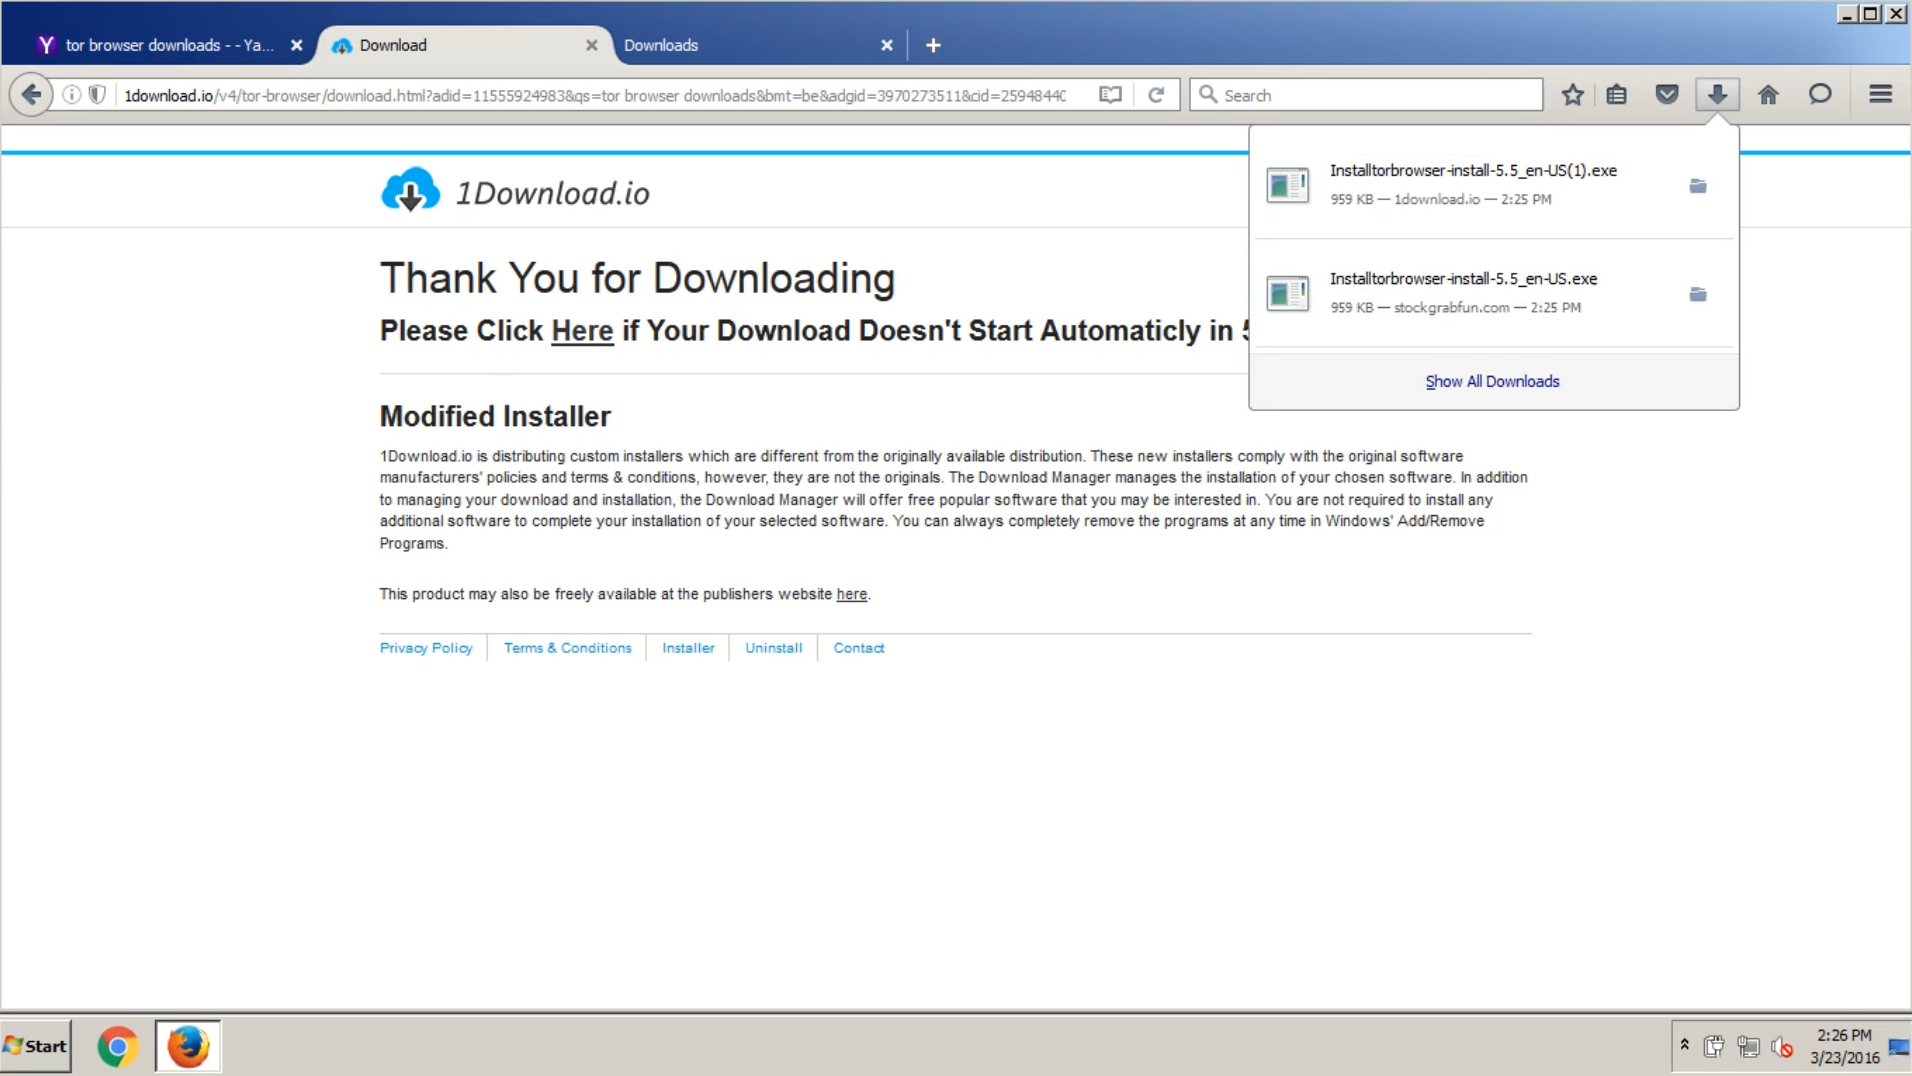
\includegraphics[width=0.5\textwidth]{../experiment/processing/bad-participants/X10-20160323-132505-1downloadio.png}
\caption{E2-OLD-X10-20160323-1400 attempted to download Tor Browser from TechSpot.com, but clicked on
a download link which was not from TechSpot.com. The download was from another site, 1download.io.}
\label{downloadio}
\end{figure} 

\begin{figure}
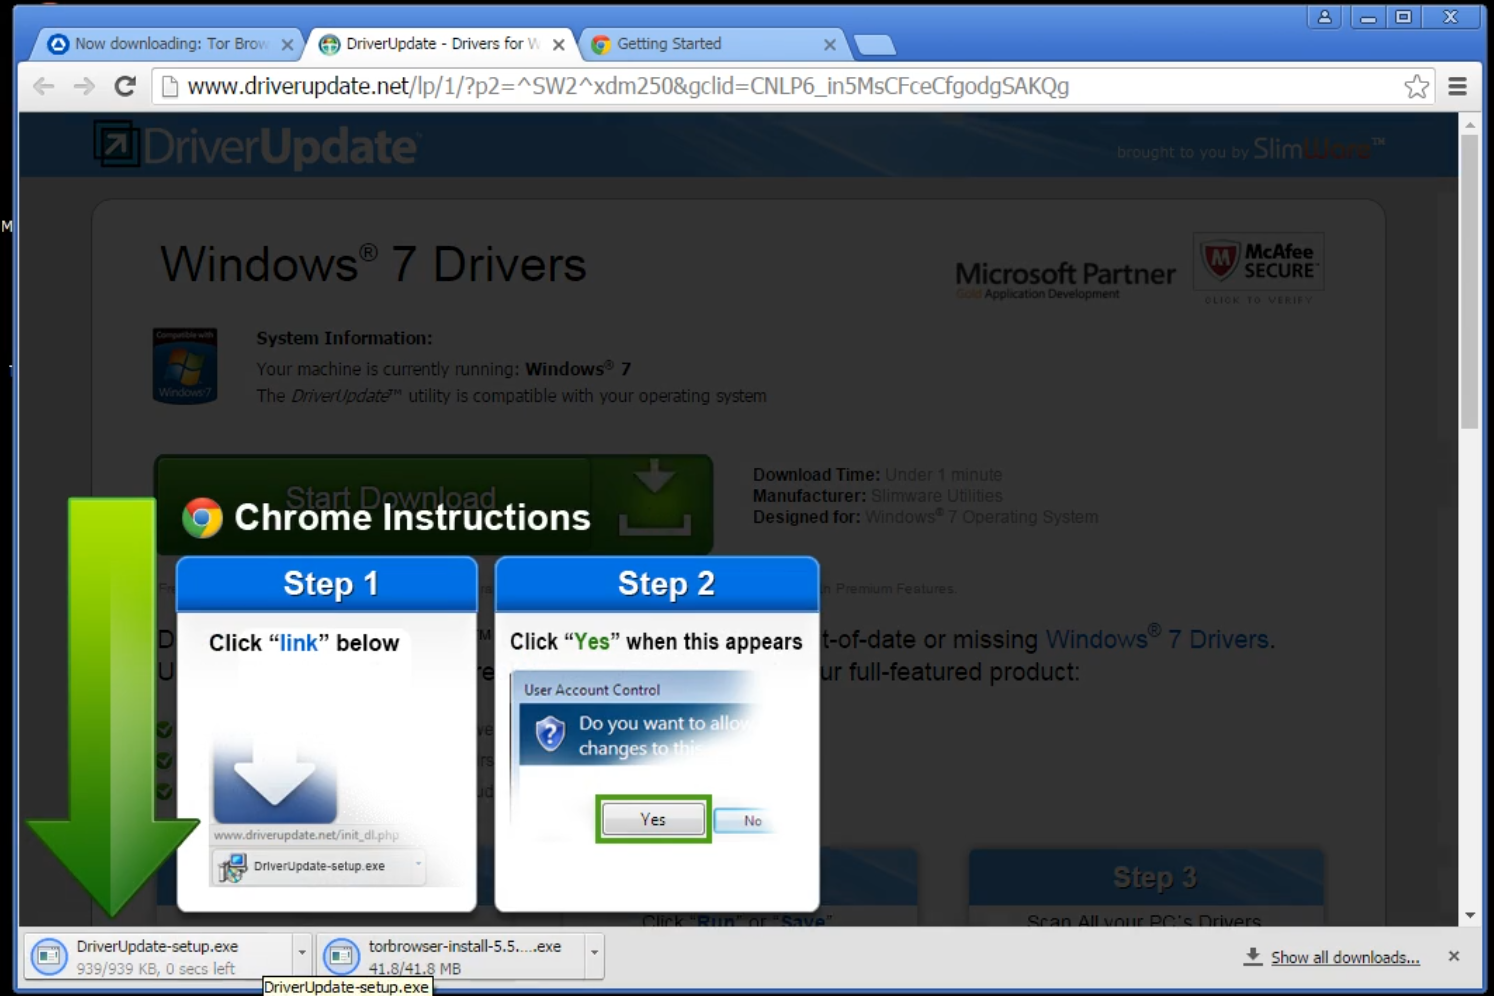
\includegraphics[width=0.5\textwidth]{../experiment/processing/bad-participants/X28-20160328-134111-driverupdate.png}
\caption{E2-OLD-X28-20160328-1400 downloaded Tor Browser from DriverUpdate, a suspicious source. Two executables
are downloaded, and the website instructs the user to run an executable named ``DriverUpdate-setup.exe,'' which the
participant dutifully does before running the Tor Browser executable.}
\label{driverupdate}
\end{figure} 

\begin{figure}
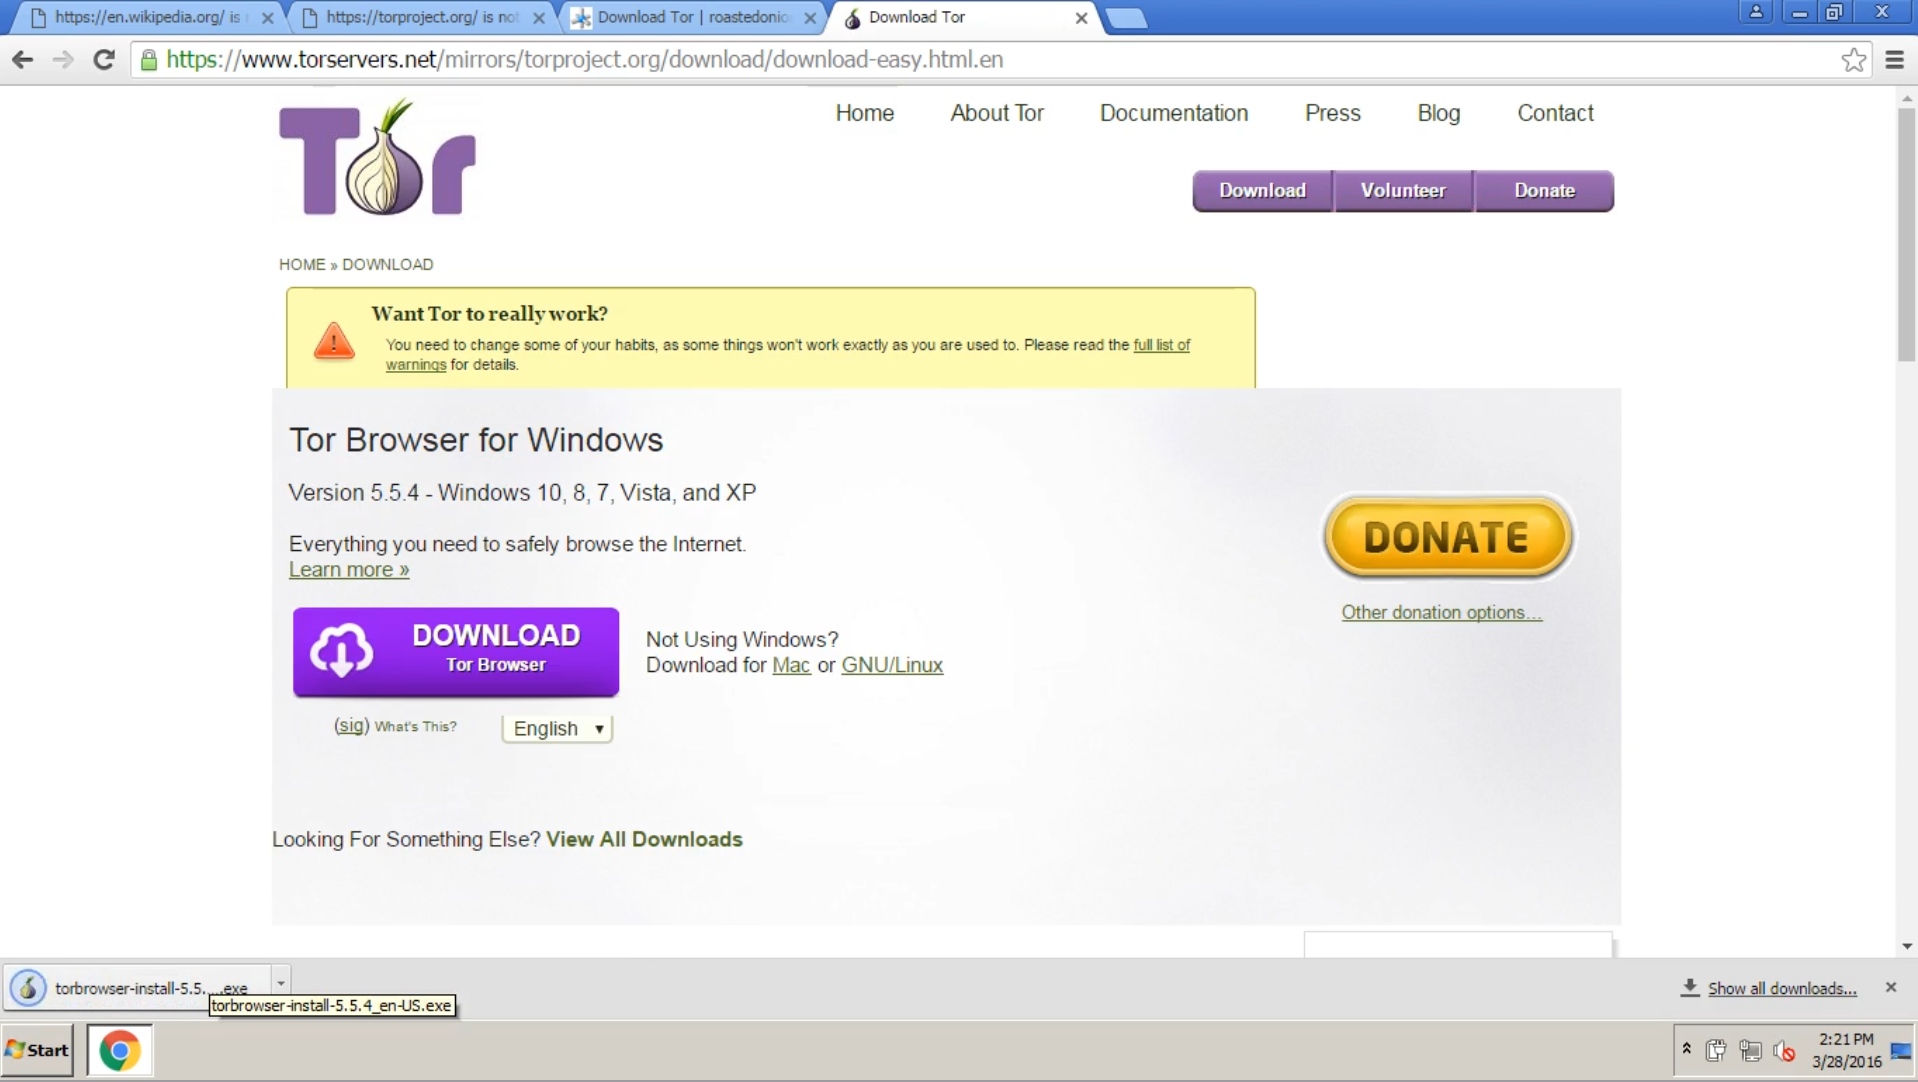
\includegraphics[width=0.5\textwidth]{../experiment/processing/bad-participants/X32-20160328-134531-mirror.png}
\caption{E1-OLD-X32-20160328-1400 downloaded Tor Browser from a legitimate Tor Browser mirror, \url{www.torservers.net/mirrors}.}
\label{mirror}
\end{figure}

\begin{figure}
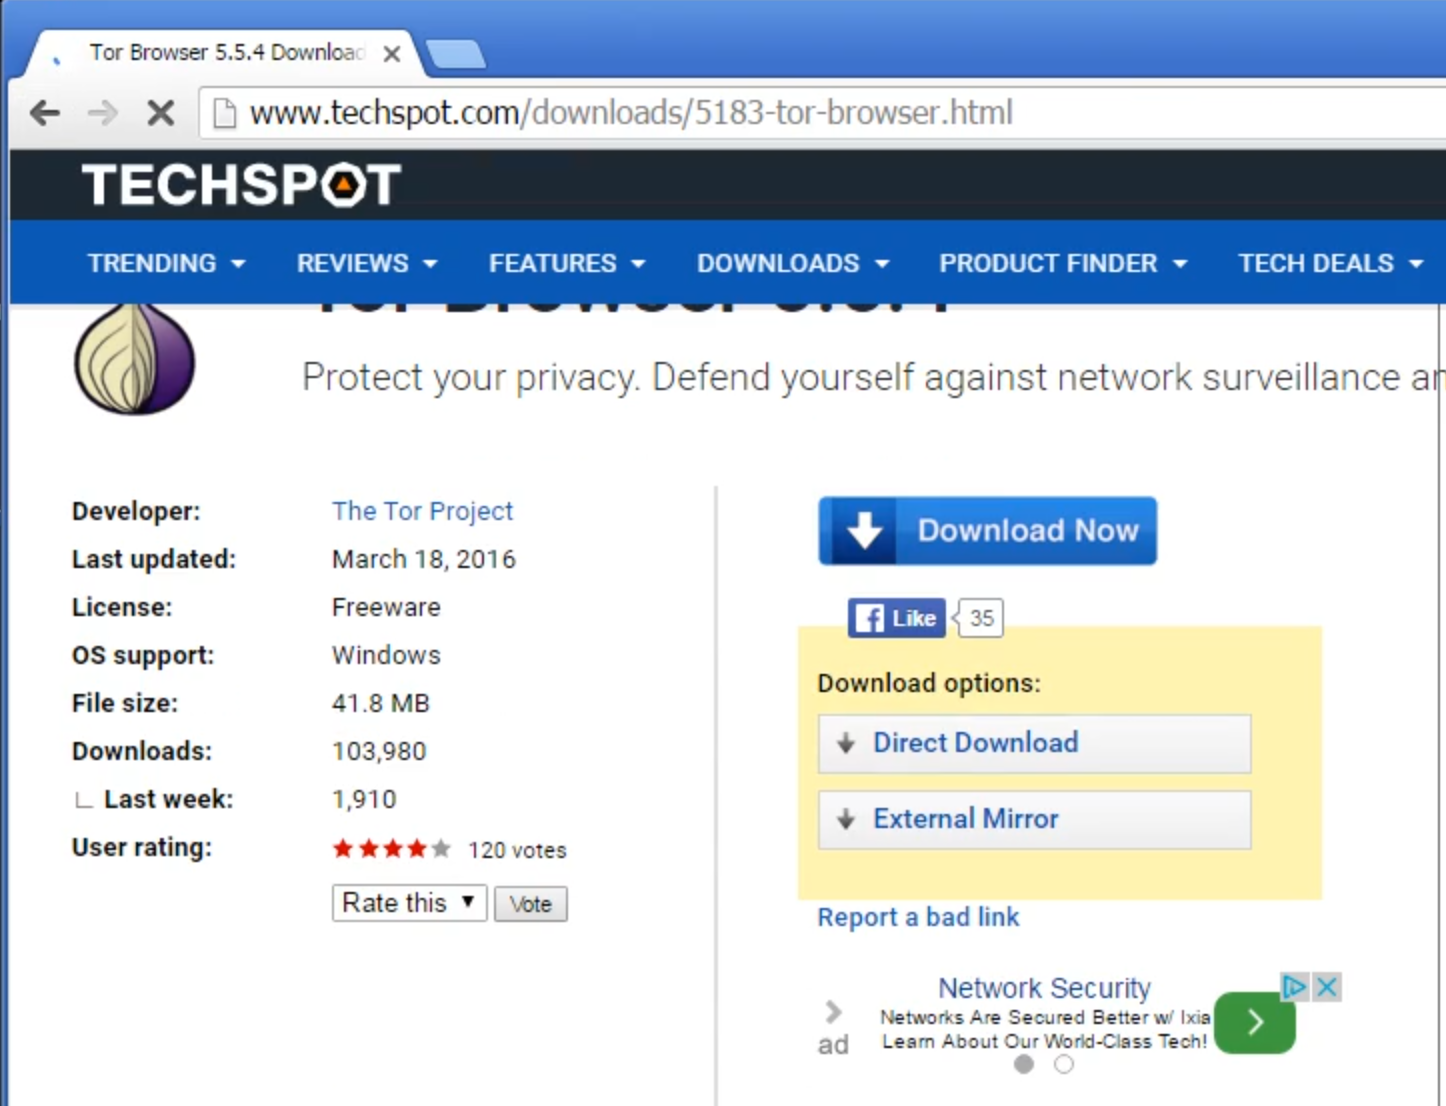
\includegraphics[width=0.5\textwidth]{../experiment/processing/bad-participants/20160323-133257-techspot.png}
\caption{E2-NEW-X21-20160323-1400 downloaded Tor Browser from TechSpot, clicking on the download link from 
TechSpot (the white ``Direct Download'' button). X10-20160323-132505 in Fig.~\ref{downloadio} clicked the blue ``Download Now'' button and downloaded from a different source.}
\label{techspot}
\end{figure}

\begin{figure}
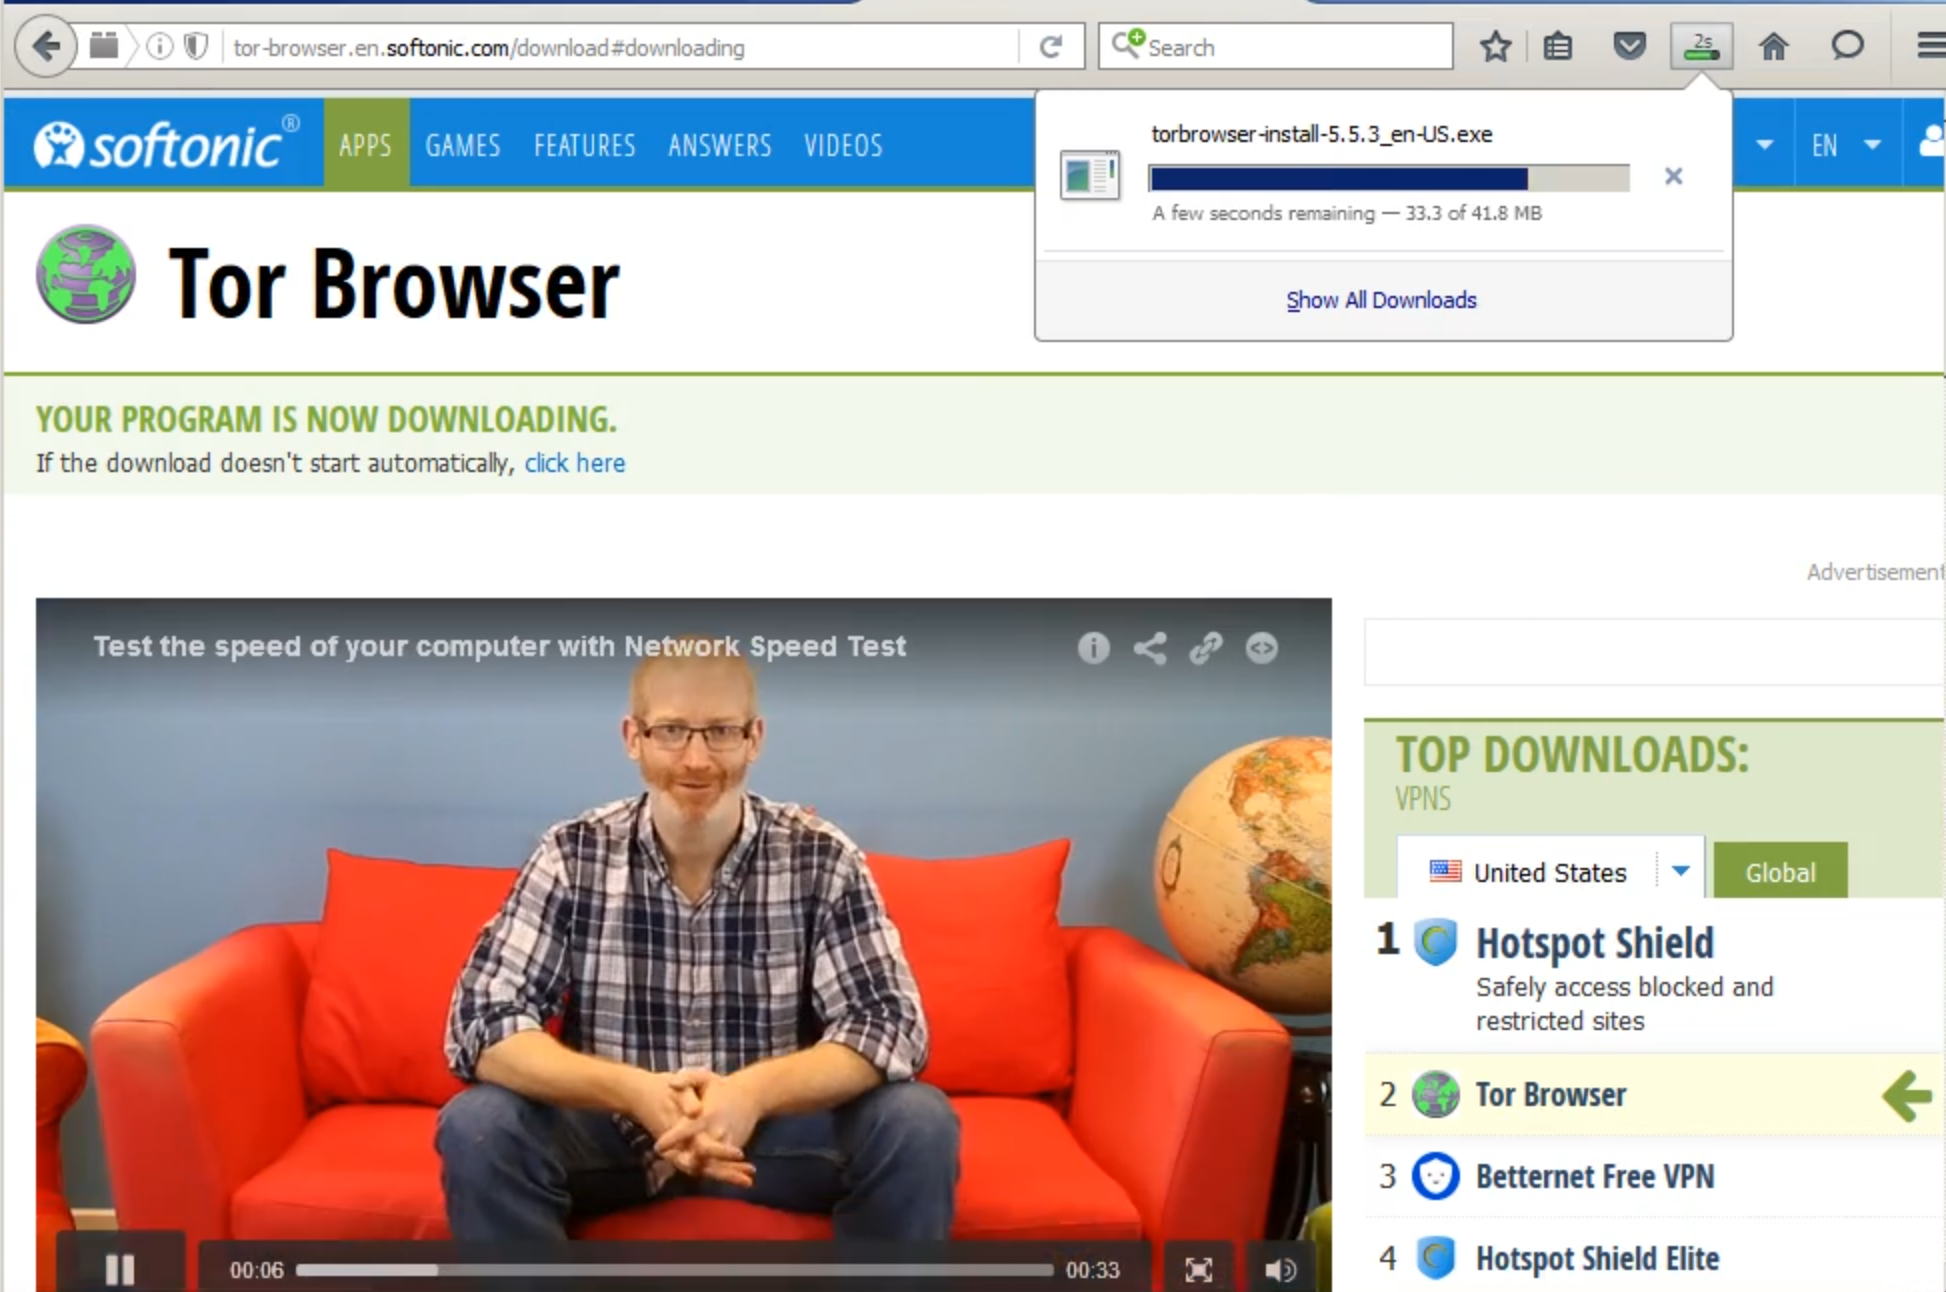
\includegraphics[width=0.5\textwidth]{../experiment/processing/bad-participants/20160330-161511-softsonic.png}
\caption{E3-NEW-X11-20160330-1600 downloaded Tor Browser from Softsonic, a reputable-looking but
unconfirmed site.}
\label{softsonic}
\end{figure}



\end{document}
